\documentclass[reprint,prb,superscriptaddress]{revtex4-2}
\usepackage{braket,amsmath,graphicx,color}
\usepackage{hyperref}
\bibliographystyle{apsrev4-1}
\begin{document}

\title{Local metal-insulator transition in a generalised impurity Anderson model}
\author{Abhirup Mukherjee}
\email{am18ip014@iiserkol.ac.in }
\affiliation{Department of Physical Sciences, Indian Institute of Science Education and Research-Kolkata, W.B. 741246, India}
\author{Siddhartha Lal}
\email{slal@iiserkol.ac.in}
\affiliation{Department of Physical Sciences, Indian Institute of Science Education and Research-Kolkata, W.B. 741246, India}

\date{\today}

\begin{abstract}
Lorem ipsum dolor sit amet, consectetur adipiscing elit, sed do eiusmod tempor incididunt ut labore et dolore magna aliqua. Ut enim ad minim veniam, quis nostrud exercitation ullamco laboris nisi ut aliquip ex ea commodo consequat. Duis aute irure dolor in reprehenderit in voluptate velit esse cillum dolore eu fugiat nulla pariatur. Excepteur sint occaecat cupidatat non proident, sunt in culpa qui officia deserunt mollit anim id est laborumLorem ipsum dolor sit amet, consectetur adipiscing elit, sed do eiusmod tempor incididunt ut labore et dolore magna aliqua. Ut enim ad minim veniam, quis nostrud exercitation ullamco laboris nisi ut aliquip ex ea commodo consequat. Duis aute irure dolor in reprehenderit in voluptate velit esse cillum dolore eu fugiat nulla pariatur. Excepteur sint occaecat cupidatat non proident, sunt in culpa qui officia deserunt mollit anim id est laborumLorem ipsum dolor sit amet, consectetur adipiscing elit, sed do eiusmod tempor incididunt ut labore et dolore magna aliqua. Ut enim ad minim veniam, quis nostrud exercitation ullamco laboris nisi ut aliquip ex ea commodo consequat. Duis aute irure dolor in reprehenderit in voluptate velit esse cillum dolore eu fugiat nulla pariatur. Excepteur sint occaecat cupidatat non proident, sunt in culpa qui officia deserunt mollit anim id est laborum
\end{abstract}

\maketitle

%\tableofcontents

\section{Introduction}

The Hubbard model is one of the fundamental models for strong electronic correlation; in its simplest form, it features a single band of conduction electrons hopping on a lattice and interacting via local correlations that provide a cost \(U\) if any site is doubly occupied. There are two trivial limits of the model. At \(U=0\), the bath consists of just a kinetic energy part, and the ground state is just a filled Fermi sea. At \(t=0\), each lattice site decouples from the rest and becomes a local moment, which under symmetry-breaking becomes a Neel antiferromagnet. This suggests that on increasing \(U/t\) beyond some critical value, the system might undergo a phase transition from a metallic state to an insulating state~\cite{Mott_1949}. This transition is reflected in the local spectral function - while it has a well-defined zero energy peak in the metallic phase, it is gapped in the insulating phase.

One method of studying Hubbard models is through auxiliary models, described in the next section. Auxiliary models are simpler versions of the full Hamiltonian that are able to capture the essential physics. For eg, a correlated impurity interacting with a conduction bath is a potential auxiliary model for the Hubbard Hamiltonian:
The impurity has onsite energy \(\epsilon_d\) and an onsite correlation \(U\). It hybridises into the bath through \(V\).

If the impurity site hybridises with a {\it non-interacting} bath defined by a uniform density of states, the impurity spectral function is found to have a well-defined Kondo resonance at low temperatures. Increasing the impurity correlation \(U\) only serves to reduce the width of the central peak at the cost of the appearance of side bands at energy scales of the order of \(U\), but the resonance never dies. The situation is however different if the impurity is embedded in a correlated conduction bath with a non-trivial density of states. For the case of a conduction band with the DOS shown in the right of the figure below, the impurity hybridises into a reduced bandwidth because of the correlation on the lattice~\cite{held_2013}.

This difference in the type of conduction baths is utilized in dynamical mean-field theory to describe various phases of the bulk system.
This is done through the DMFT algorithm: one starts with a non-interacting bath, but depending on the value of \(U\), the conduction bath then gets modified and we ultimately end up with something that is different from what we started with.
For small \(U\), the bath does not change much and we retain the central resonance of the impurity spectral function.
This then describes a metal in the bulk.
For larger values of \(U\), however, the bath changes significantly such that its density of states becomes non-constant.
Above a critical \(U_c\), the impurity spectral function gets gapped out, and that then describes the insulating phase in the bulk.
\textit{This leaves open the following question}: What is the minimal correlation one can insert into the non-interacting bath (of a single-impurity Anderson model) that can capture both the metallic and insulating phases of the bulk model?

\begin{figure}[!htb]
\centering
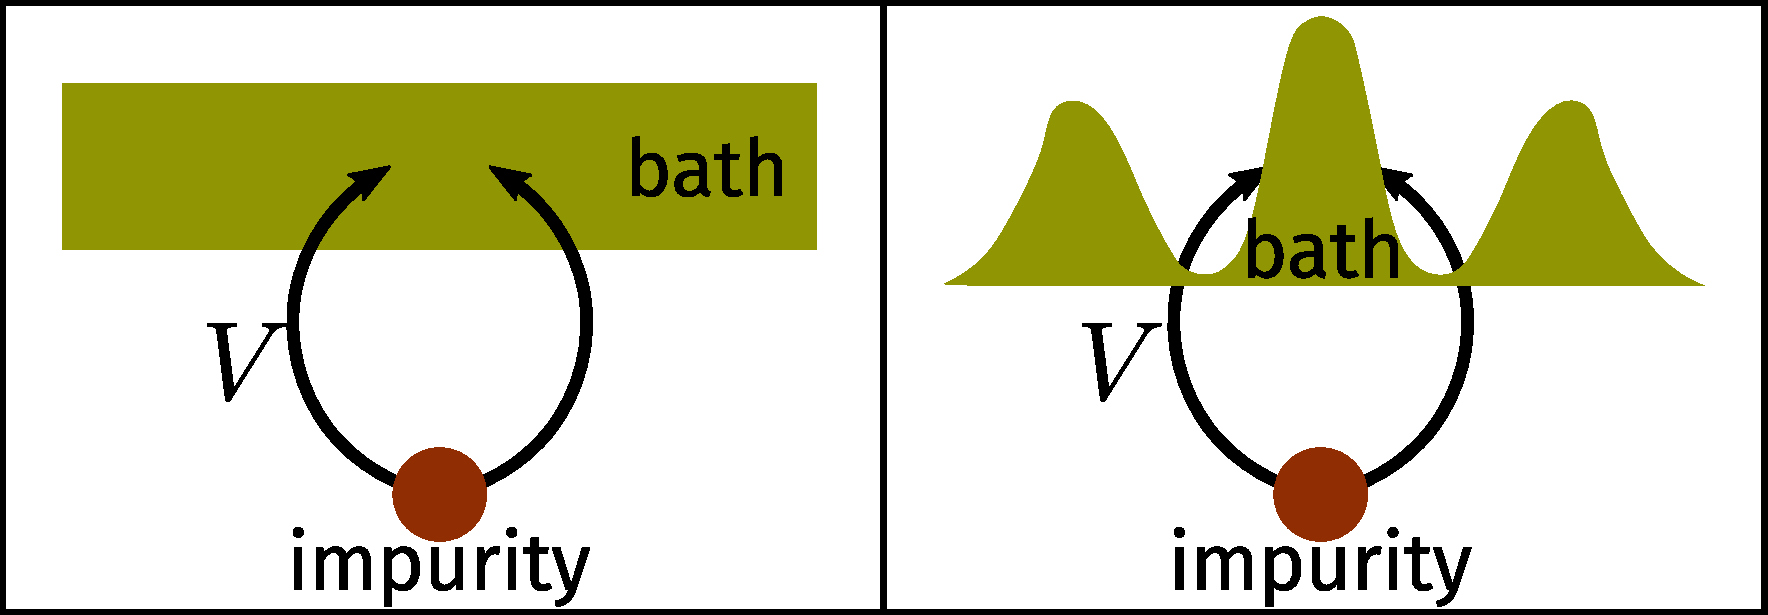
\includegraphics[width=0.5\textwidth]{../figures/dos_diff.pdf}
\caption{Two kinds of bath that an impurity can hybridise into. The left panel shows a non-interacting conduction band with a flat density of states. The right panel shows an interacting bath with an energy-dependent density of states. In the latter case, the impurity "feels" a reduced effective bandwidth defined by the width of the central peak.}
\end{figure}

Lorem ipsum dolor sit amet, consectetur adipiscing elit, sed do eiusmod tempor incididunt ut labore et dolore magna aliqua. Ut enim ad minim veniam, quis nostrud exercitation ullamco laboris nisi ut aliquip ex ea commodo consequat. Duis aute irure dolor in reprehenderit in voluptate velit esse cillum dolore eu fugiat nulla pariatur. Excepteur sint occaecat cupidatat non proident, sunt in culpa qui officia deserunt mollit anim id est laborum
Lorem ipsum dolor sit amet, consectetur adipiscing elit, sed do eiusmod tempor incididunt ut labore et dolore magna aliqua. Ut enim ad minim veniam, quis nostrud exercitation ullamco laboris nisi ut aliquip ex ea commodo consequat. Duis aute irure dolor in reprehenderit in voluptate velit esse cillum dolore eu fugiat nulla pariatur. Excepteur sint occaecat cupidatat non proident, sunt in culpa qui officia deserunt mollit anim id est laborum
Lorem ipsum dolor sit amet, consectetur adipiscing elit, sed do eiusmod tempor incididunt ut labore et dolore magna aliqua. Ut enim ad minim veniam, quis nostrud exercitation ullamco laboris nisi ut aliquip ex ea commodo consequat. Duis aute irure dolor in reprehenderit in voluptate velit esse cillum dolore eu fugiat nulla pariatur. Excepteur sint occaecat cupidatat non proident, sunt in culpa qui officia deserunt mollit anim id est laborum
Lorem ipsum dolor sit amet, consectetur adipiscing elit, sed do eiusmod tempor incididunt ut labore et dolore magna aliqua. Ut enim ad minim veniam, quis nostrud exercitation ullamco laboris nisi ut aliquip ex ea commodo consequat. Duis aute irure dolor in reprehenderit in voluptate velit esse cillum dolore eu fugiat nulla pariatur. Excepteur sint occaecat cupidatat non proident, sunt in culpa qui officia deserunt mollit anim id est laborum
Lorem ipsum dolor sit amet, consectetur adipiscing elit, sed do eiusmod tempor incididunt ut labore et dolore magna aliqua. Ut enim ad minim veniam, quis nostrud exercitation ullamco laboris nisi ut aliquip ex ea commodo consequat. Duis aute irure dolor in reprehenderit in voluptate velit esse cillum dolore eu fugiat nulla pariatur. Excepteur sint occaecat cupidatat non proident, sunt in culpa qui officia deserunt mollit anim id est laborumLorem ipsum dolor sit amet, consectetur adipiscing elit, sed do eiusmod tempor incididunt ut labore et dolore magna aliqua. Ut enim ad minim veniam, quis nostrud exercitation ullamco laboris nisi ut aliquip ex ea commodo consequat. Duis aute irure dolor in reprehenderit in voluptate velit esse cillum dolore eu fugiat nulla pariatur. Excepteur sint occaecat cupidatat non proident, sunt in culpa qui officia deserunt mollit anim id est laborumLorem ipsum dolor sit amet, consectetur adipiscing elit, sed do eiusmod tempor incididunt ut labore et dolore magna aliqua. Ut enim ad minim veniam, quis nostrud exercitation ullamco laboris nisi ut aliquip ex ea commodo consequat. Duis aute irure dolor in reprehenderit in voluptate velit esse cillum dolore eu fugiat nulla pariatur. Excepteur sint occaecat cupidatat non proident, sunt in culpa qui officia deserunt mollit anim id est laborum




\section{The generalised Anderson impurity model}

The impurity models we will work with couple the impurity to a single site in the lattice. We will refer to that specific site as the zeroth site throughout. We recall the Hamiltonian of the Anderson impurity model (AIM) with a half-filled impurity site:
\begin{equation} 
	\mathcal{H} = \frac{- U}{2} \left(\hat n_{d \uparrow} - \hat n_{d \downarrow}\right)^2 + \sum_{\vec k,\sigma} \epsilon_{\vec k} \tau_{\vec k,\sigma} + V\sum_\sigma \left( c^\dagger_{d\sigma}c_{0\sigma} + \text{h.c.}\right)~,
 \end{equation}
where \(\tau_{\vec k,\sigma} \equiv \hat n_{\vec k,\sigma} - 1/2\). Also, \(c_{d\sigma}\) and \(c_{0\sigma}\) are the fermionic annihilation operators of spin \(\sigma\) for the impurity and zeroth sites respectively. \(U\) is the repulsive correlation on the impurity site, and the impurity is at particle-hole symmetry. \(V\) is the momentum-independent hybridisation parameter that couples the impurity with the lattice. We will work with a constant density of states in the bath. 

In order to enhance the Anderson impurity model (AIM), we introduce two extra two-particle interaction terms into the Hamiltonian:
\begin{itemize}
	\item a spin-exchange term \(J \vec{S}_d\cdot\vec{s}_0\) between the impurity spin \(\vec S_d\) and the spin \(\vec s_0\) of the zeroth site 
	\item a local particle-hole symmetric correlation term \(-U_b \hat n_{0 \uparrow} \hat n_{0 \downarrow}\) on the zeroth site
\end{itemize}

With these additional terms, the {\it generalised Anderson impurity model} (henceforth referred to as the GAIM), at particle-hole symmetry, is
\begin{equation}\begin{aligned}
	\label{GIAM-ham}
	\mathcal{H} = -\frac{1}{2}U \left(\hat n_{d \uparrow} - \hat n_{d \downarrow}\right)^2 + \sum_{\vec k,\sigma} \epsilon_{\vec k} \tau_{\vec k,\sigma} + J \vec{S}_d\cdot\vec{s}_0 \\
	+ V\sum_\sigma \left( c^\dagger_{d\sigma}c_{0\sigma} + \text{h.c.}\right) - U_b \hat n_{0 \uparrow} \hat n_{0 \downarrow}
\end{aligned}\end{equation}
All the terms in the Hamiltonian have been depicted schematically in Fig.~\ref{zeromode-bare}.

\begin{figure}[!htb]
	\centering
	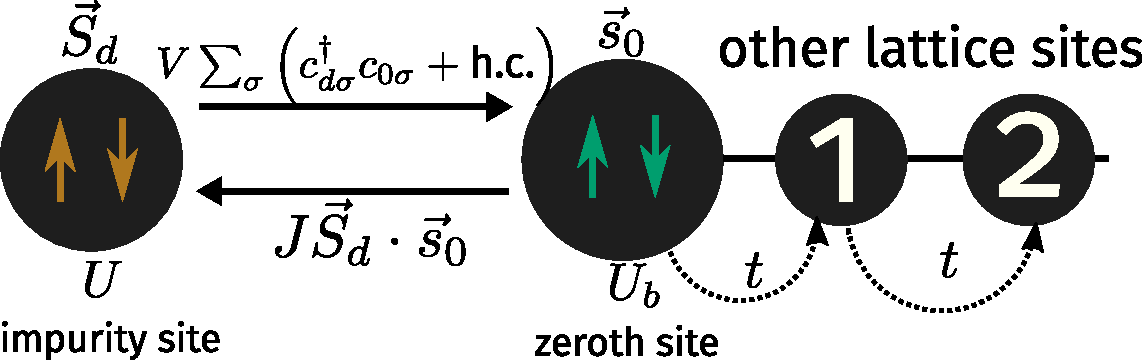
\includegraphics[width=0.45\textwidth]{../figures/zeromode_bare.pdf}
	\caption{While we have studied the full model under renormalisation group, often we will turn to a simplified zero-bandwidth version of the model that is obtained by ignoring the kinetic energy part of the Hamiltonian. This zero-bandwidth model is effectively a two site model.}
	\label{zeromode-bare}
\end{figure}

\section{Method and RG Equations}

\subsection{The unitary RG method}
The focus here is on obtaining the low-energy phases of the GAIM. To accomplish this, we perform a renormalisation group analysis of the associated Hamiltonian (eq.~\ref{GIAM-ham}) using the recently developed unitary renormalisation group (URG) method \cite{anirbanmott1,anirbanmott2,anirbanurg1,anirbanurg2,siddharthacpi,santanukagome,1dhubjhep,Mukherjee_mott_merg,anirban_kondo}. The unitary RG transformations lead to a series of Hamiltonians \(H_{(j)}\) related to the Hamiltonian at the previous step through a unitary transformation; the unitary transformations are defined by the requirement that they remove number fluctuations in high-energy \(k-\)states, thus making the Hamiltonian progressively more block-diagonal in momentum space. The high-energy degrees of freedom that get decoupled in the process become integrals of motion (IOMs) for the Hamiltonian and enter the Hamiltonian only in a purely number-diagonal form.

To be more precise, we first choose a complete basis \(\left\{ \ket{j} \right\} \) and arrange these states from high-energy (UV) to low-energy (IR). Typically we take these states to be the momentum eigenstates \(\left(\ket{j} = \left\{\ket{\vec k \uparrow}, \ket{\vec k \downarrow}\right\}\right)\), and the isoenergetic shells \(\left\{D_{(j)}\right\}\) then define the sequence of states, such that the momenta far away from the Fermi surface (taken to be at higher \(j\) and having \(|D_{(j)}| \gg |\epsilon_F|\)) are taken to be the UV states while those near the Fermi surface (taken to be at lower \(j\) and having \(D_{(j)} \sim \epsilon_F\)) comprise the IR states. This scheme is shown in Fig.~\ref{urg-scheme}.

\begin{figure}[htpb]
	\centering
	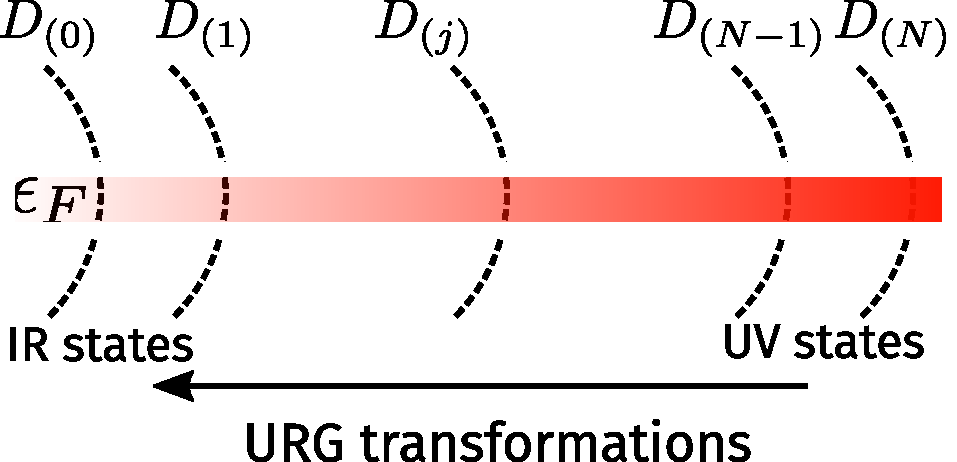
\includegraphics[width=0.45\textwidth]{../figures/urg-scheme.pdf}
	\caption{High energy - low energy scheme defined and used in the URG method. The states away from the Fermi surface form the UV subspace and are decoupled first, leading to a Hamiltonian which is more block-diagonal and comprised of only the IR states near the Fermi surface.}
	\label{urg-scheme}
\end{figure}

At a given RG step \(j\), the Hamiltonian \(H_{(j)}\) involves number fluctuations between the \(k-\)states that have energies lower than \(D_{(j+1)}\). So the most energetic states that are still non-trivially present in \(H_{(j)}\) are those on the energy contour \(D_{(j)}\), and the Hamiltonian \(H_{(j)}\) will, in general, not conserve the number of particles in this energy (or momentum) state: \(\left[H_{(j)}, \hat n_{j}\right] \neq 0\). The unitary transformation \(U_{(j)}\) is then defined so as to remove this number fluctuation at the next RG step~\cite{anirbanurg1,anirbanurg2}:
\begin{equation}\begin{aligned}
	H_{(j-1)} = U_{(j)} H_{(j)} U^\dagger_{(j)}~, ~\left[H_{(j-1)}, \hat n_{j}\right] =0~.
\end{aligned}\end{equation}

The unitary transformations can be expressed in terms of a generator \(\eta_{(j)}\) that has fermionic algebra~\cite{anirbanurg1,anirbanurg2}:
\begin{equation}\begin{aligned}
	U_{(j)} = \frac{1}{\sqrt 2}\left(1 + \eta_{(j)} - \eta_{(j)}^\dagger\right)~,~ \quad\left\{ \eta_{(j)},\eta_{(j)}^\dagger \right\}_\pm = 1~,
\end{aligned}\end{equation}
where \(\left\{A,B\right\}_\pm = AB \pm BA\). The generator itself is given by the expression~\cite{anirbanurg1,anirbanurg2}
\begin{equation}\begin{aligned}
	\eta^\dagger_{(j)} = \frac{1}{\hat \omega_{(j)} - \text{Tr}\left(H_{(j)} \hat n_{j}\right) } c^\dagger_{j} \text{Tr}\left(H_{(j)}c_{j}\right)~.
\end{aligned}\end{equation}
The important operator \(\hat \omega_{(j)}\) originates from the quantum fluctuations that exist in the problem because of the non-commutation of the kinetic energy terms and the interaction terms in the Hamiltonian:
\begin{equation}\begin{aligned}
	\hat \omega_{(j)} = H_{(j-1)} - H^i_{(j)}~.
\end{aligned}\end{equation}
\(H^i_{(j)}\) is the part of \(H_{(j)}\) that commutes with \(\hat n_j\) but does {\it not} commute with at least one \(\hat n_l\) for \(l < j\). The RG flow continues up to energy \(D^*\), where a fixed point is reached from the vanishing of the RG function. 

\subsection{URG equations for the GAIM}

The derivation of the RG equations for the generalised Anderson impurity model (GAIM) Hamiltonian is shown in the appendix. We provide below the RG equations for a given quantum fluctuation scale \(\omega\):
\begin{gather}
	\Delta U_b = 0~,\\
	\Delta U = 4V^2 n_j\left(\frac{1}{d_1} - \frac{1}{d_0}\right) - n_j\frac{J^2}{d_2}~,\\
	\Delta V = -\frac{3n_j V}{8}\left[J\left(\frac{1}{d_2} + \frac{1}{d_1}\right) +  \frac{4U_b}{3}\sum_{i=1}^4 \frac{1}{d_i}\right]~,\\
	\Delta J = -\frac{n_j J\left(J + 4U_b\right)}{d_2}~.
\end{gather}
The denominators \(d_i\) used in these equations are given by
\begin{gather}
	d_0 = \omega - \frac{D}{2} + \frac{U_b}{2} - \frac{U}{2}~,d_2 = \omega - \frac{D}{2} + \frac{U_b}{2} + \frac{J}{4}~,\\
	d_1 = \omega - \frac{D}{2} + \frac{U_b}{2} + \frac{U}{2} + \frac{J}{4}~,d_3 = \omega - \frac{D}{2} + \frac{U_b}{2}~.
\end{gather}
The symbols used in the RG equations have the following meanings: \(\Delta U\) represents the renormalisation in the coupling \(U\) in going from the \(j^\text{th}\) Hamiltonian to the \(\left( j-1 \right) ^\text{th}\) Hamiltonian by decoupling the isoenergetic shell at energy \(D_{(j)}\). \(n_j\) is the number of electronic states on the shell \(D_{(j)}\).

We will discuss the consequences of these RG equations in the next sections, but we clarify here that the labels \(U_0,J_0,V_0\) that might occur in the figures or elsewhere in the text represent the bare values of the associated couplings \(U,J\) and \(V\). We also point out here that throughout the upcoming results, the bare value of \(U_b\) is set to the negative of the bare value of \(U_0\): \(U_b = -U_0/10\). This means that whenever we vary \(U_0\) along the axis of a plot, we are simultaneous varying \(U_b\). The reason for choosing the negative sign of \(U_b\) will be clarified in the next section.

\section{RG flows and phase diagram}

We start the discussion on the nature of the RG flows by noting that the bath correlation \(U_b\) is marginal, and the spin-exchange coupling \(J\) has a critical point \(\left( \Delta J = 0 \right) \) at \(r \equiv -U_b/J = 1/4 \equiv r_c\). We will look at the RG flows of the couplings \(U,V\) and \(J\) on both sides of this critical point by tuning the ratio \(r\) across the critical value \(r_c\), and see what phases they lead to. We will work in the regime of quantum fluctuations where all the denominators are negative: \(d_i < 0 ~\forall~i\). Before we start, note that:
\begin{itemize}
	\item Since \(J\) is positive, this means that we can capture both relevant and irrelevant RG flows of \(J\) by keeping \(U_b\) negative. \(U_b\) is found to be marginal under the RG transformation, and we set \(U_b\) to \(-U_0/10\) hereafter.
	\item The critical point has been chosen from the RG equation of \(J\) and not of \(V\); this is because, the RG irrelevance of \(J\) is sufficient to make \(V\) irrelevant as well, and on the other hand, the RG relevance of \(J\) is sufficient to screen the impurity.
\end{itemize}
  

\subsection{RG flows for \(r < r_c\)}

In this regime, \(J\) is relevant and flows to large positive values. It is also easy to deduce from its RG equation that \(V\) is also relevant. \(U\) is more non-trivial, because its RG equation involves both \(V\) and \(J\). Nevertheless, the RG equations were solved numerically with bare values of the couplings and the bandwidth, and it was found that while \(V\) and \(J\) are relevant, \(U\) is irrelevant. These findings are shown in the blue curves of Fig.~\ref{rg-flow}. The fixed point values can be summarised as:
\begin{equation}\begin{aligned}
	U^* = 0, ~ ~ ~ ~ V^* \gg 1, ~ ~ ~ ~ J^* \gg 1, ~ ~ ~ ~ U_b \sim \mathcal{O}(1)
\end{aligned}\end{equation}


\subsection{RG flows for \(r > r_c\)}

The RG \(\beta\)-function function for \(J\) changes sign as \(r\) grows greater than \(r_c\) upon tuning \(U_b\) to less than \(-J_0/4\), and \(J\) becomes irrelevant. As for \(V\), note that in the RG equation for \(V\), it is \(J\) that drives \(V\) to be relevant while \(U_b\) drives \(V\) to irrelevance; if \(J\) itself is irrelevant, then \(\Delta V\) will be dominated by \(U_b\) and \(V\) will be ultimately irrelevant. The behaviour of \(U\) is again non-trivial and analytically not tractable, so we solve the RG equations numerically. It turns out that although \(U\) is slightly irrelevant, it saturates to an appreciable value near the fixed point. These RG flows are shown in the purple curves of Fig.~\ref{rg-flow}. The fixed point values in this regime can be summarised as:
\begin{equation}\begin{aligned}
	U^* \sim \mathcal{O}(1), ~ ~ ~ ~ V^* =0, ~ ~ ~ ~ J^* =0, ~ ~ ~ ~ U_b \sim \mathcal{O}(1)
\end{aligned}\end{equation}

\begin{figure}[!htb]
	\centering
	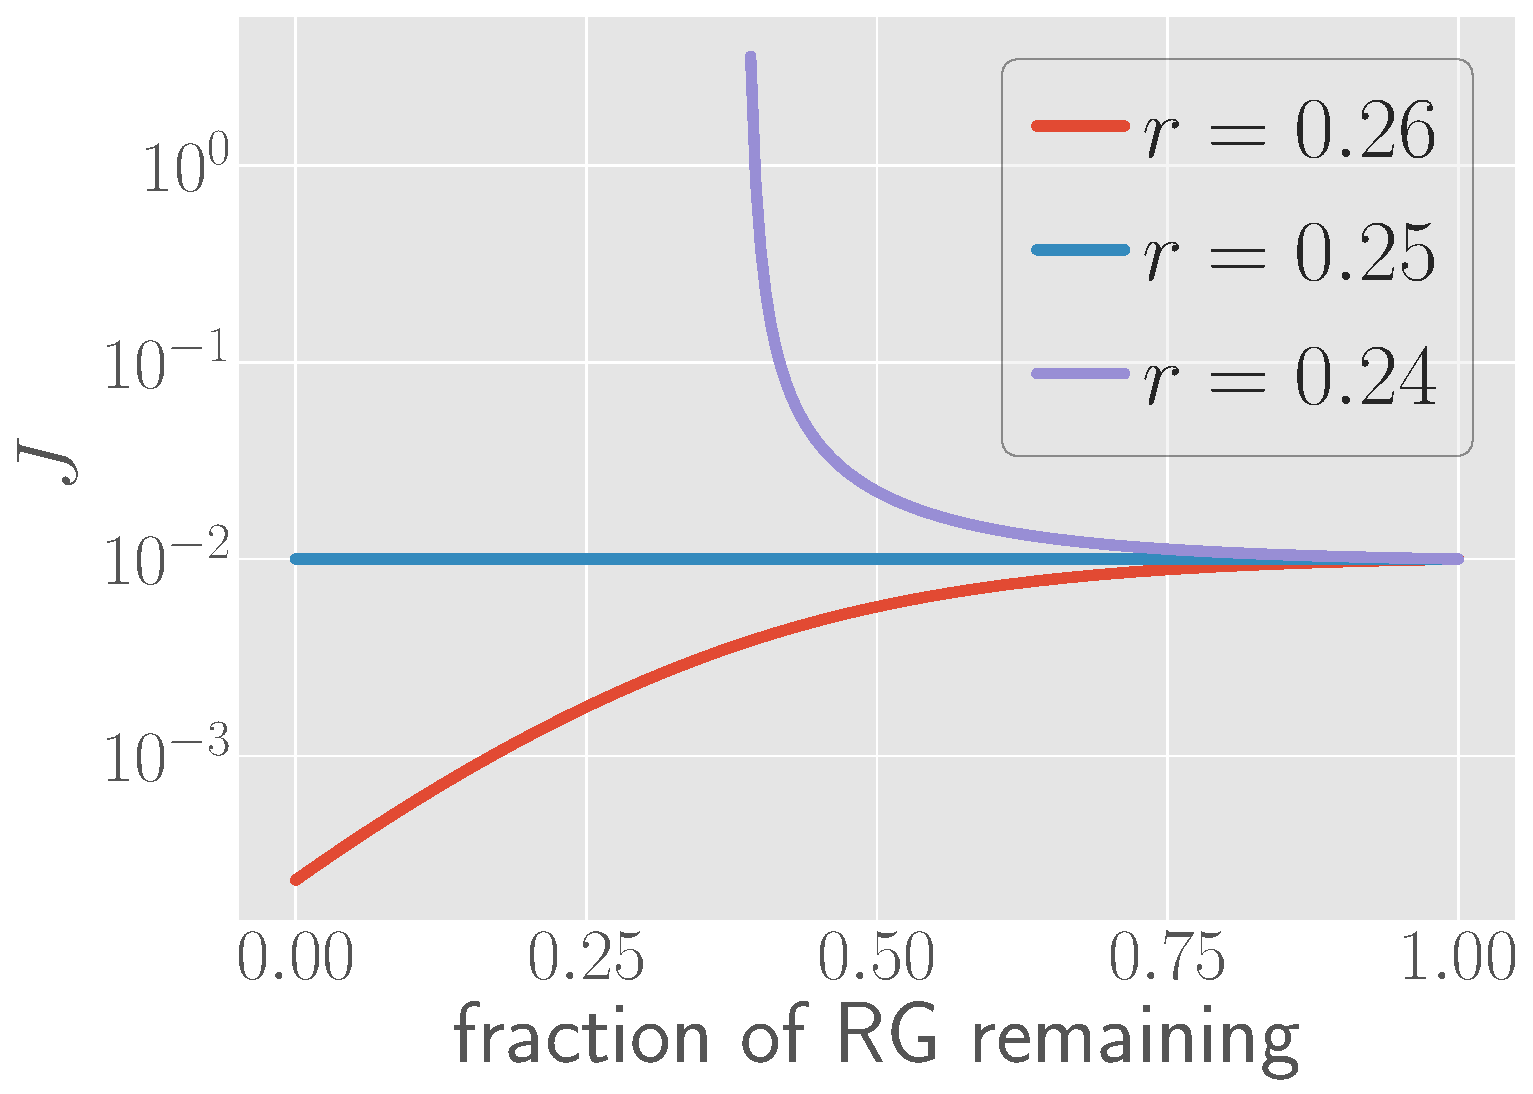
\includegraphics[width=0.48\textwidth]{../figures/J_Ub.pdf}
	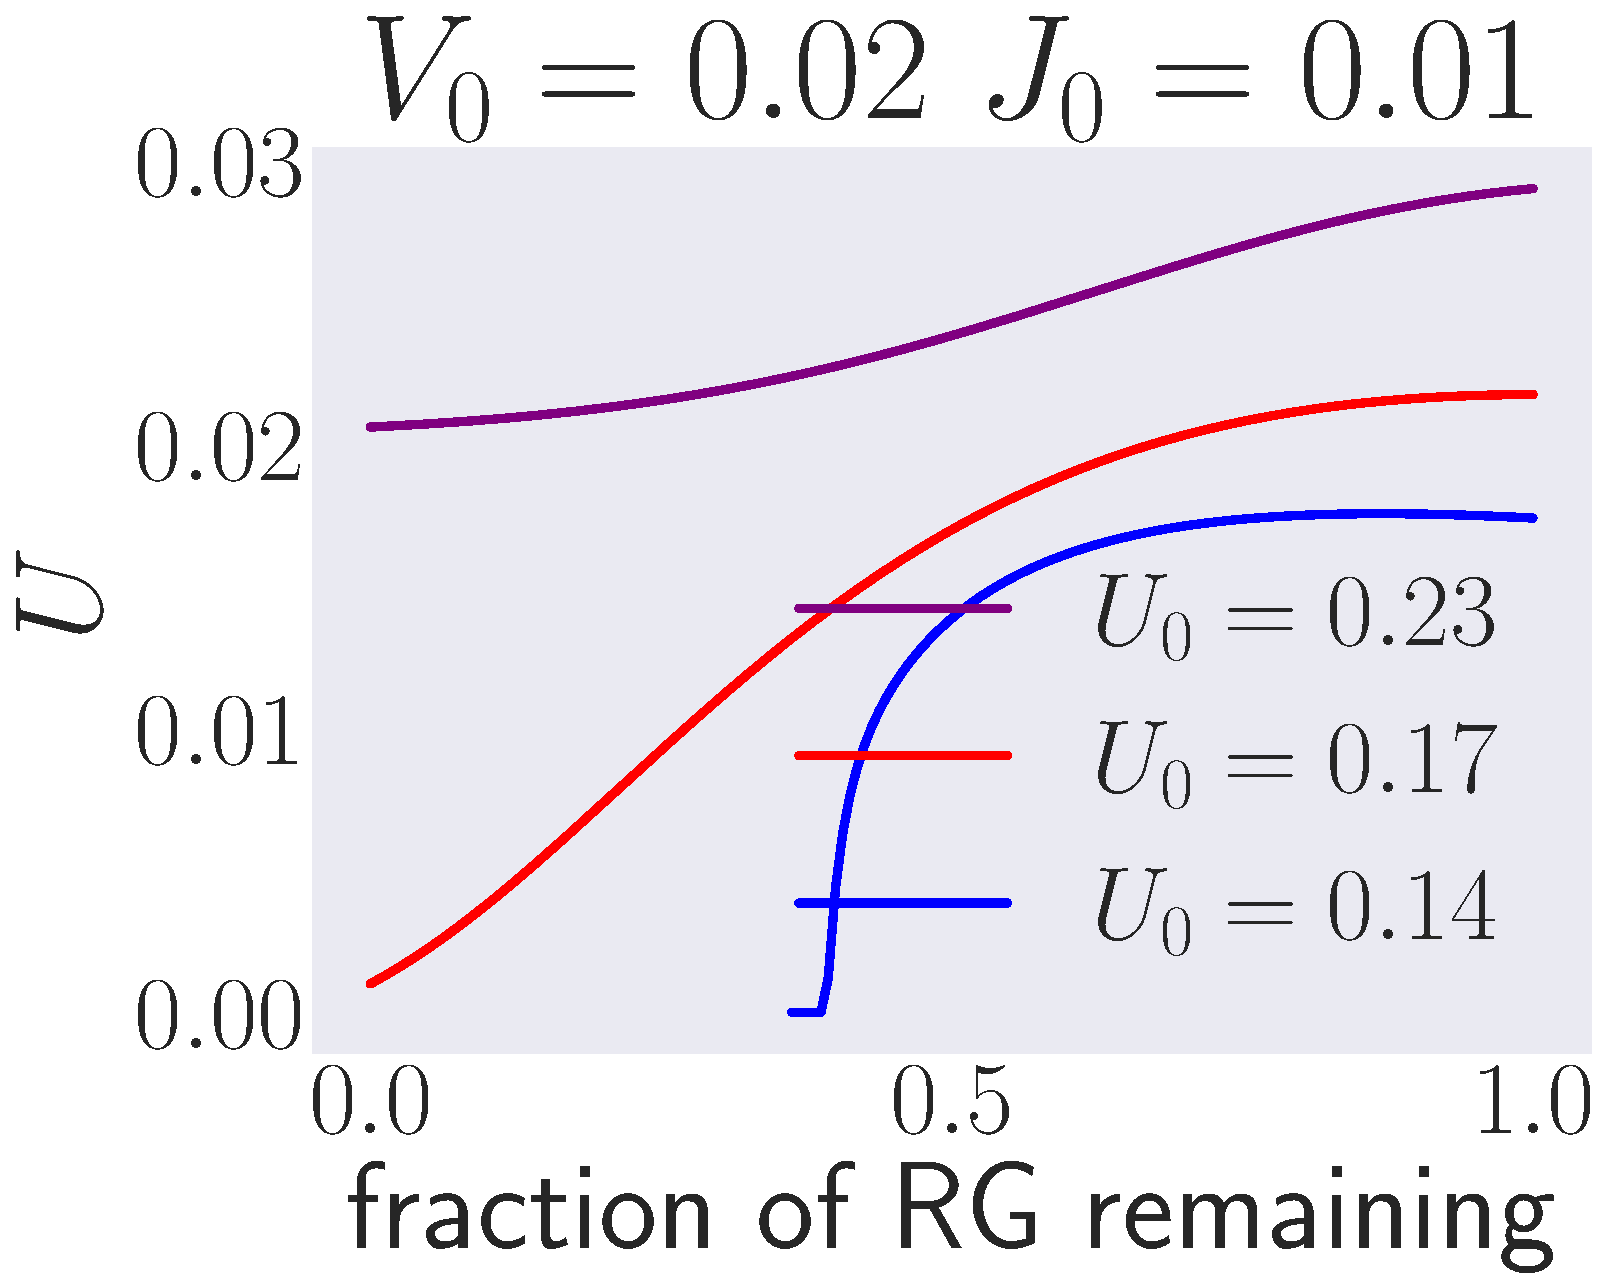
\includegraphics[width=0.48\textwidth]{../figures/U_Ub.pdf}
	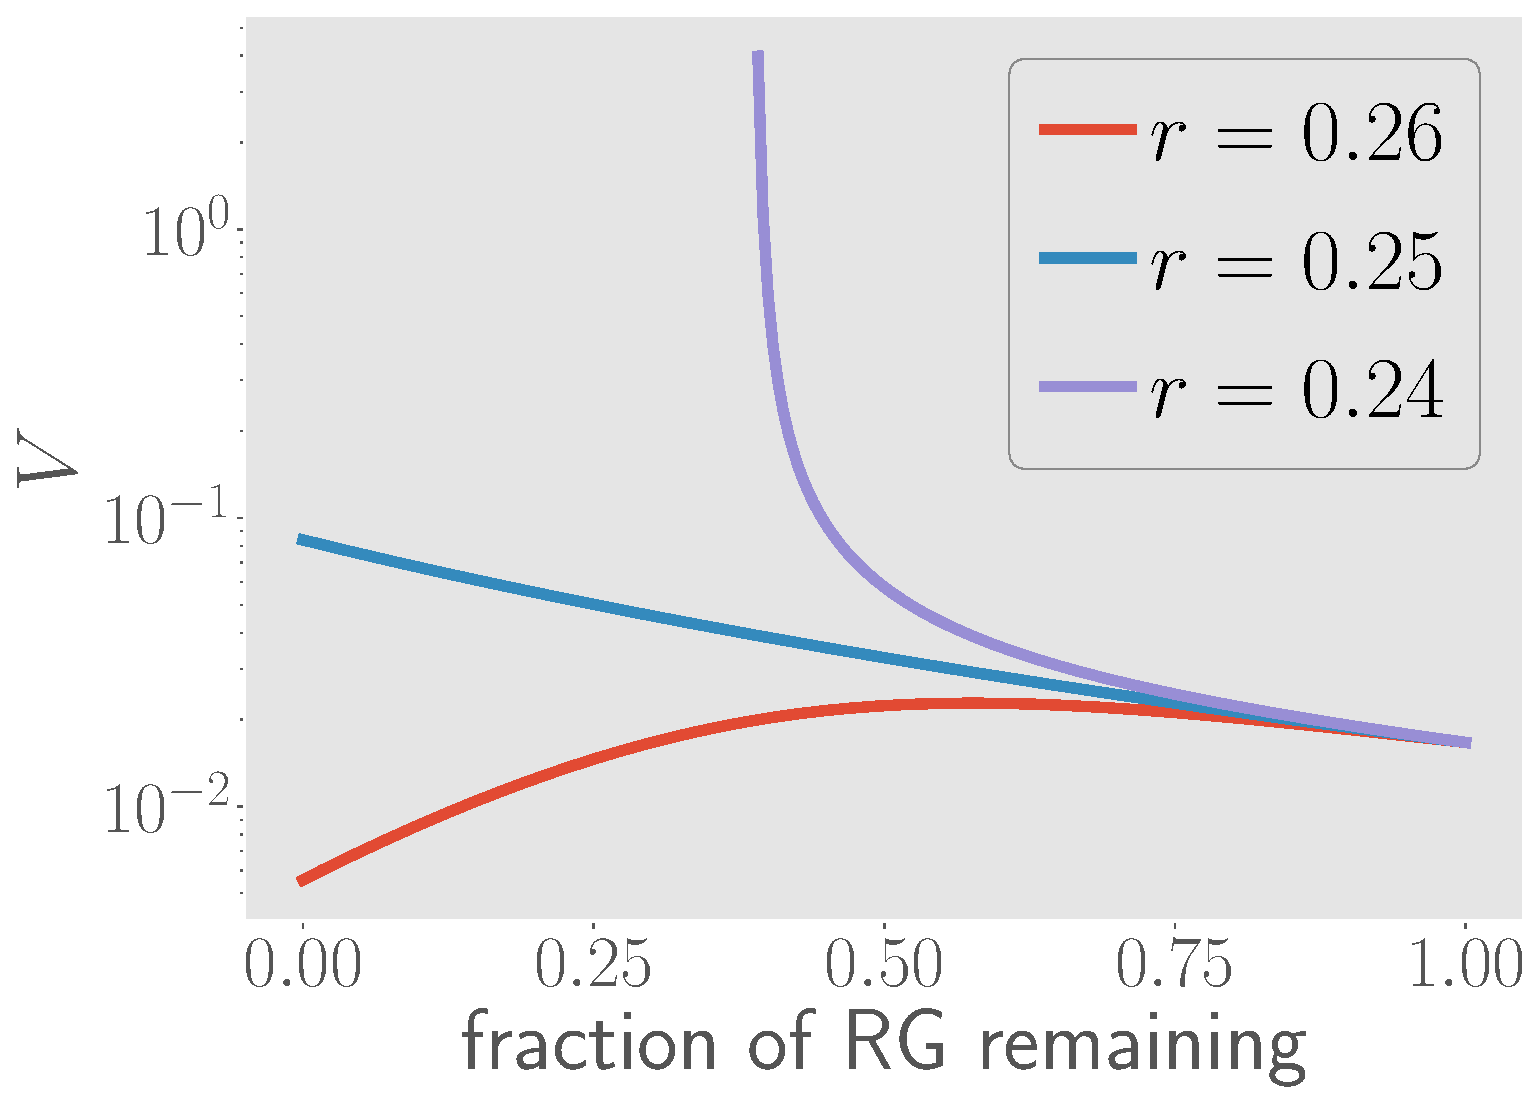
\includegraphics[width=0.48\textwidth]{../figures/V_Ub.pdf}
	\caption{Variation of couplings \(U,V\) and \(J\) along the RG transformations, for three values of the transition-tuning ratio \(r\). x-axis represents the RG steps, the rightmost point is the first RG step and leftmost point is the final RG step. The values of the bare couplings are given in the title. All values are in units of the half-bandwidth \(D_0\), which is chosen to be 10. The blue curves represent the flows for \(r > r_c\), where \(J\) is relevant. The purple curves represent the RG flows for \(r < r_c\), where \(J\) is irrelevant. The red curves are exactly at the critical point \(r = r_c\), where \(J\) is marginal.}
	\label{rg-flow}
\end{figure}

\subsection{Phase diagram: impurity phase transition}

The low-energy RG phase diagram is obtained by solving the RG equations for ranges of couplings, and is shown in Fig.~\ref{phase-diag}. There are four distinct phases in the space of couplings \(U_0 \text{ vs } J_0\), with \(U_b\) constrained at \(-U_0/10\) and \(V_0\) set to \(2J_0\). The red phase (phase A in the legend) is composed of those Hamiltonians which lead to RG relevant \(V,J\) and RG irrelevant \(U\). In other words, this is the phase where the impurity moment is screened by the conduction electrons. This is the low-energy phase of the AIM that has \(U\) and \(V\). The blue phase (phase B in the legend) consists of those Hamiltonians which produce irrelevant \(J,V\) and a relevant \(U\); here, the conduction electrons fail to screen the impurity and a residual local moment survives on the impurity at low energies. The yellow phase (phase C in the legend) lies in between these two phases, and is defined by non-negligible \(V^*, U^*\) but zero \(J^*\). In this phase, the impurity still gets screened, but there is more charge content on the impurity site compared to phase B. On going to the thermodynamic limit by increasing the bandwidth \(D_0\), this light green phase disappears. The gray phase (phase D in the legend) is a ``dead" phase where \(U,V,J\) are all RG irrelevant. The various phases are summarised in table.~\ref{summary-phases}.

The black line in Fig.~\ref{phase-diag} represents a line of critical points \(U_b = J_0\), and separates the two major phases of the impurity. Such a {\it phase transition} between the screened impurity and the local moment phases is absent in the AIM without the attractive correlation \(U_b\). In fact, only the purple screened phase is adiabatically connected the AIM.

\begin{table}[!htb]
\centering
\begin{tabular}{|c|c|c|}
\hline
phase & RG flow & fixed point \\ 
\hline
A & \(\Delta U <0, ~ ~ \Delta J,\Delta V>0\) & \(U^* \ll V^* \ll J^*\) \\ 
B &  \(\Delta U > 0, ~ ~ \Delta J,\Delta V<0\) & \(U^* \gg 1, ~ ~V^*, J^* = 0\)\\
C &  \(\Delta U, \Delta J < 0,~ ~\Delta V>0\) & \(J^* < U^* \ll V^*\) \\
D &  \(\Delta U, \Delta J,\Delta V < 0\) & \(U^*, V^*, J^* = 0\) \\
\hline
\end{tabular}
\caption{Summary of the various fixed point phases}
\label{summary-phases}
\end{table}

\begin{figure}[!htb]
	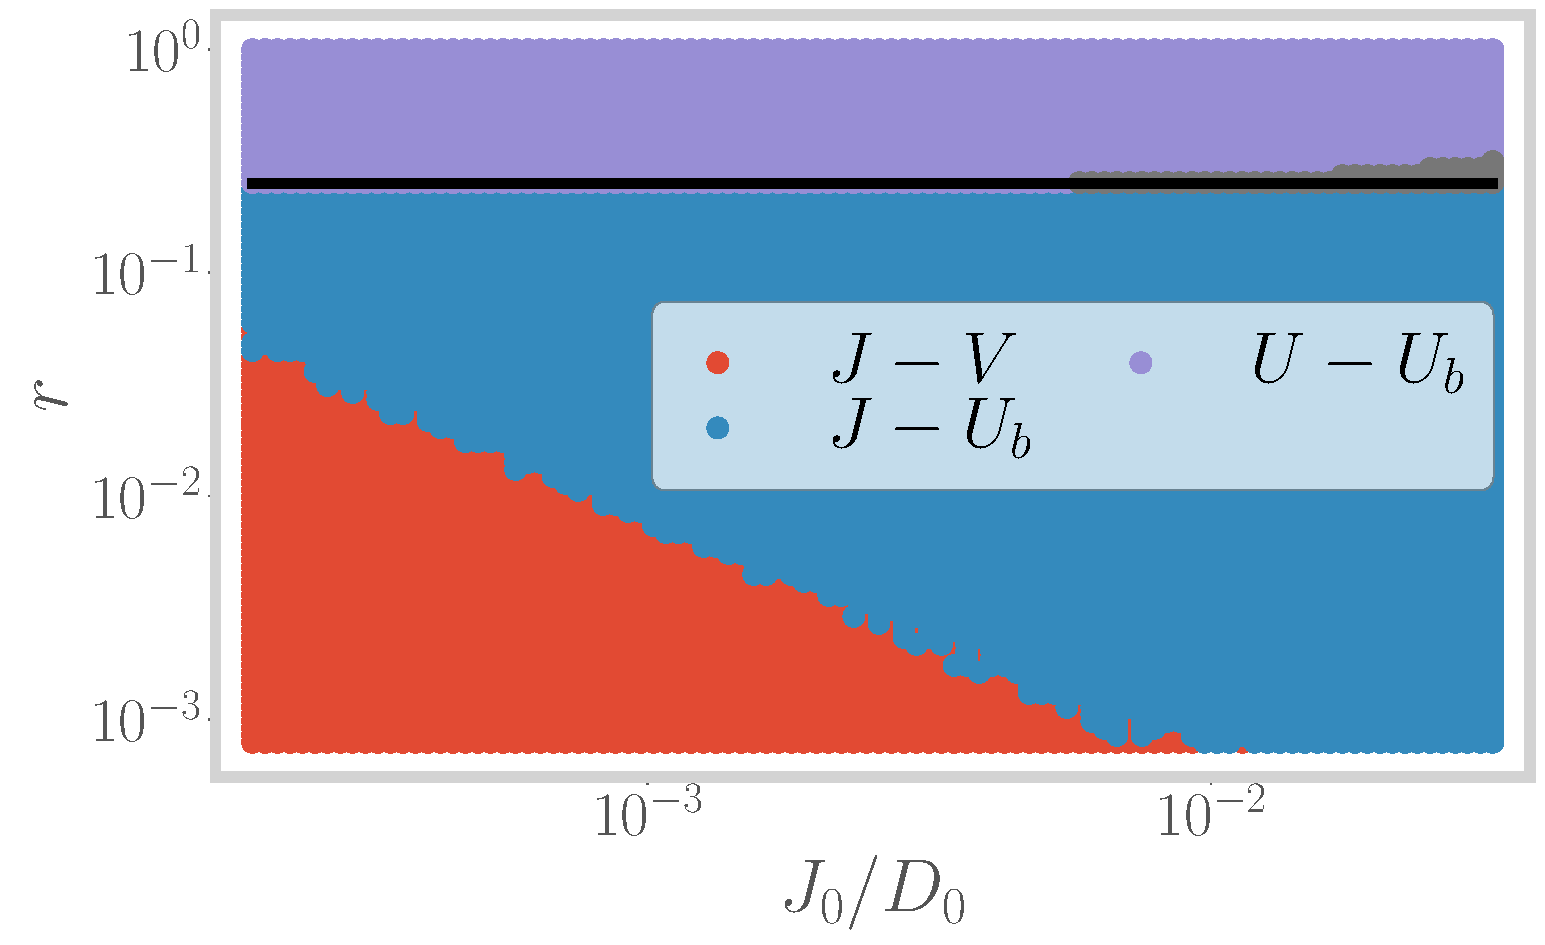
\includegraphics[width=0.5\textwidth]{../figures/phase-map-MIT.pdf}
	\caption{Phase diagram of the GAIM, in the space of couplings \(U_0\) and \(J_0\). \(U_b\) is set to \(-U_0/10\) and \(V_0\) is set to \(2J_0\). The various phases \(A\) through \(D\) are characterised in the text.}
	\label{phase-diag}
\end{figure}

\section{Low-energy effective Hamiltonian and the ground state}

The RG fixed point Hamiltonian describes the low-energy phase of the system. In general, if the RG fixed point is reached at an energy scale \(D^*\), the fixed point Hamiltonian \(\mathcal{H}^*\) is obtained simply from the fixed point values of the couplings, and by noting that the states above \(D^*\) are now part of the IOMs:
\begin{equation}\begin{aligned}
	\mathcal{H}^* = -\frac{1}{2}U^*\left(\hat n_{d \uparrow} - \hat n_{d \downarrow}\right)^2 + \sum_{\sigma,\vec k:|\epsilon_{\vec k}| < D^*} \epsilon_{\vec k} \tau_{\vec k,\sigma} - U_b^* \hat n_{0 \uparrow} \hat n_{0 \downarrow} \\
	+ V^*\sum_\sigma \left( c^\dagger_{d\sigma}c_{0\sigma} + \text{h.c.}\right) + J^* \vec{S}_d\cdot\vec{s}_0
\end{aligned}\end{equation}

\subsection{Screened regime}
\(U\) is irrelevant in this regime. Moreover, as we go towards the thermodynamic limit by increasing the bandwidth \(D_0\), we find that \(J^* \gg V^*\) (see Fig.~\ref{J_bandwidth}), and the fixed point Hamiltonian is determined purely by the spin-exchange part; combining this with the local bath correlation \(U_b\) that is marginal then gives the low-energy Hamiltonian for the screened regime:
\begin{equation}
	H_\text{eff}^\text{sc} = J^* \vec{S}_d\cdot\vec{s}_0 - U_b \hat n_{0 \uparrow} \hat n_{0 \downarrow} + \sum_{\sigma,\vec k:|\epsilon_{\vec k}| < D^*} \epsilon_{\vec k} \tau_{\vec k,\sigma}
\end{equation}

\begin{figure}[!htb]
	\centering
	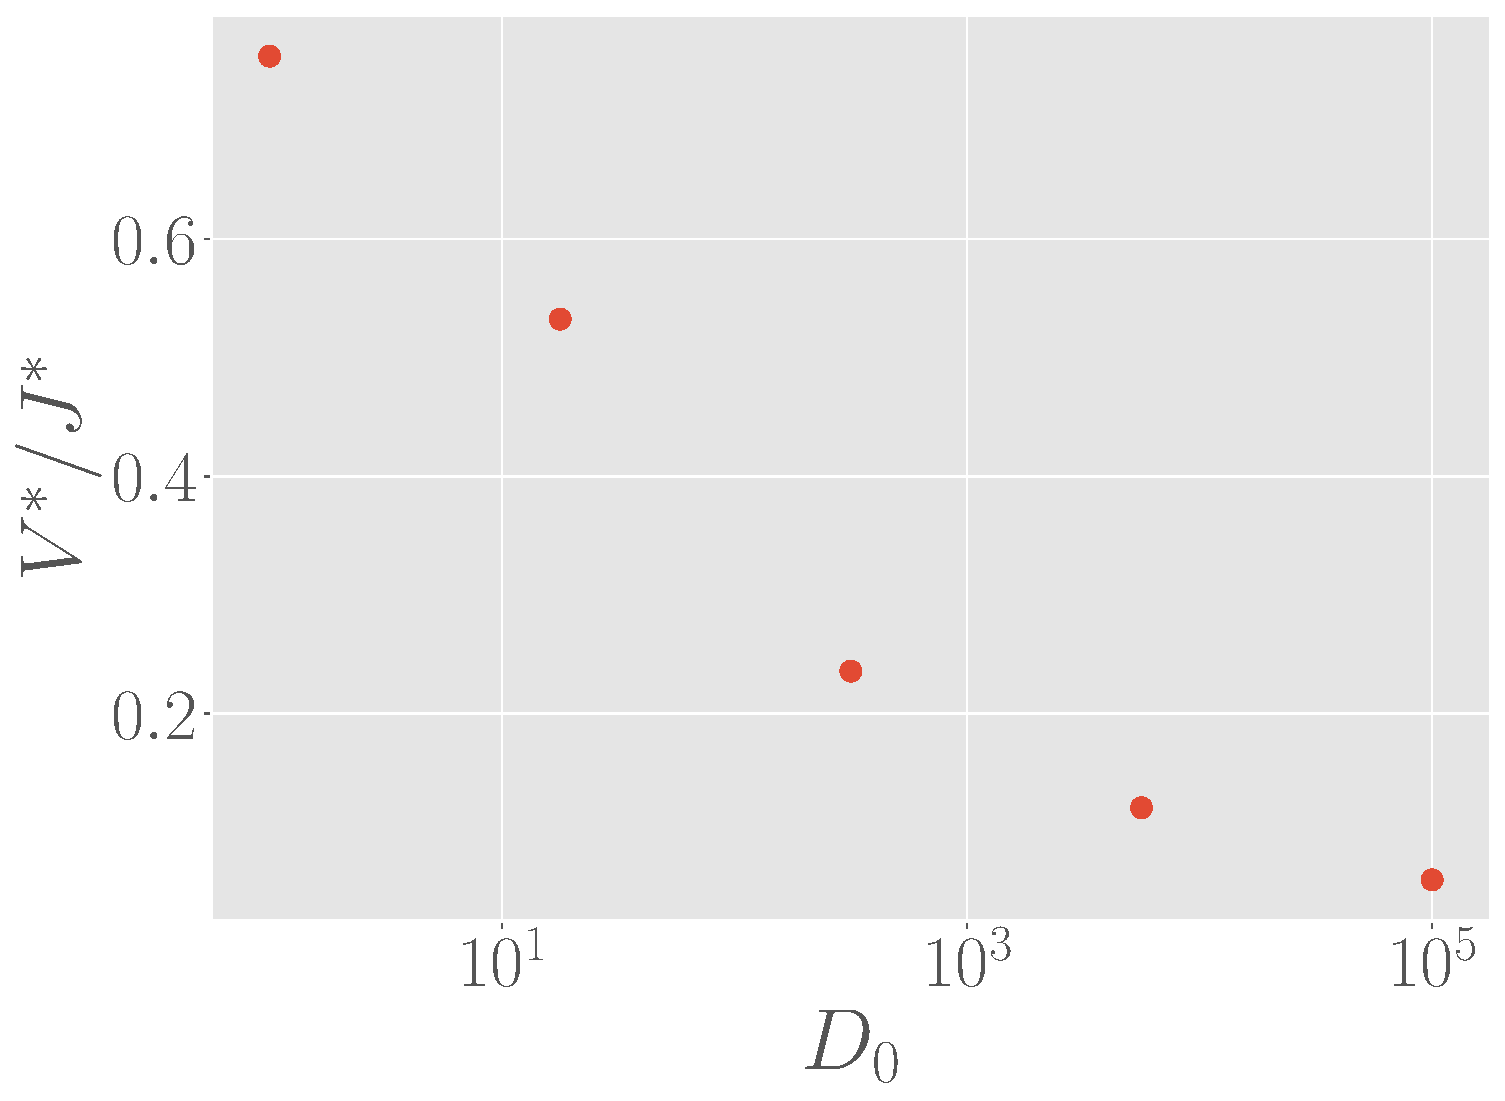
\includegraphics[width=0.5\textwidth]{../figures/J_bandwidth.pdf}
	\caption{Increase of \(J^*\) in comparison to \(V^*\) when going towards the thermodynamic limit.}
	\label{J_bandwidth}
\end{figure}

Since the high momentum modes have been decoupled, the ground state in this regime can be estimated by compressing the kinetic energy to the zero bandwidth limit: 
\begin{equation}\begin{aligned}
	\sum_{\sigma,\vec k:|\epsilon_{\vec k}| < D^*} \epsilon_{\vec k} \tau_{\vec k,\sigma} \sim \epsilon_F \sum_{\vec k_F,\sigma}\tau_{\vec k_F,\sigma}
\end{aligned}\end{equation}
Choosing the chemical potential such that \(\epsilon_F\) vanishes results in a {\it two-site Hamiltonian} composed of the impurity site and the zeroth site (see Fig.~\ref{zero-bw}):
\begin{equation}
	\label{two-site}
	H_\text{eff}^\text{sc} \sim J^* \vec{S}_d\cdot\vec{s}_0 - U_b \hat n_{0 \uparrow} \hat n_{0 \downarrow}
\end{equation}
\begin{figure}[htpb]
	\centering
	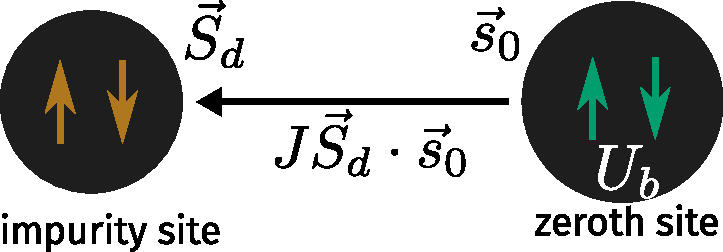
\includegraphics[width=0.5\textwidth]{../figures/zeromode_eff.pdf}
	\caption{Two site Hamiltonian obtained by taking the zero bandwidth limit of the effective Hamiltonian in the screened regime.}
	\label{zero-bw}
\end{figure}
This model is easily solved and the ground state is a maximally-entangled spin singlet formed by \(\vec S_d\) and \(\vec s_0\); the ground state energy is \(E_\text{gs}^\text{sc} = -\frac{3}{4}J^* - U_b\):
\begin{equation}\begin{aligned}
	\ket{\Psi}_\text{gs}^\text{sc} = \frac{1}{\sqrt 2}\left(\ket{\uparrow_d,\downarrow_0} - \ket{\downarrow_d,\uparrow_0}\right)
\end{aligned}\end{equation}
where \(\left\{\uparrow_d, \downarrow_d\right\}, \left\{\uparrow_0, \downarrow_0\right\}\) are the spin states of the impurity and zeroth sites respectively. As mentioned before, this regime in the GAIM is adiabatically connected to the AIM, and indeed, such a spin-singlet ground state is also obtained in the AIM from other methods like Poor Man's scaling~\cite{anderson1969exact,anderson1970}, numerical renormalisation group~\cite{wilson1975,hrk_wilson_1980}, Bethe ansatz~\cite{}, conformal field theory methods~\cite{}[CITE] and the URG analysis of the Kondo model~\cite{anirban_kondo}.

\subsection{Unscreened regime}

This regime is simpler than the screened regime, because both \(V\) and \(J\) are irrelevant, and only \(U\) is relevant. The effective Hamiltonian then consists of an impurity spin that is decoupled from the conduction bath:
\begin{equation}\begin{aligned}
	H_\text{eff}^\text{uns} = -\frac{1}{2}U^*\left(\hat n_{d \uparrow} - \hat n_{d \downarrow}\right)^2 - U_b \hat n_{0 \uparrow} \hat n_{0 \downarrow} + \sum_{\sigma,\vec k:|\epsilon_{\vec k}| < D^*} \epsilon_{\vec k} \tau_{\vec k,\sigma}
\end{aligned}\end{equation}
The impurity site has a doubly-degenerate ground state \(\left\{ \ket{\uparrow_d}.\ket{\downarrow_d}\right\}\), and the total ground state is the impurity state in direct product with the ground state \(\ket{\Psi}_\text{gs, bath}\) of the conduction bath Hamiltonian \(H_\text{eff, bath}^\text{uns} =  - U_b \hat n_{0 \uparrow} \hat n_{0 \downarrow} + \sum_{\sigma,\vec k:|\epsilon_{\vec k}| < D^*} \epsilon_{\vec k} \tau_{\vec k,\sigma}\):
\begin{equation}\begin{aligned}
	\ket{\Psi}_\text{gs}^\text{uns} = \ket{\sigma_d}\otimes\ket{\Psi}_\text{gs, bath}, ~ ~ ~ \sigma = \uparrow,\downarrow
\end{aligned}\end{equation}



\subsection{The critical point: \(4U_b + J = 0\)}

Along the critical points, \(J\) is marginal and \(U\) is irrelevant, while \(V\) is slightly relevant (see Fig.~\ref{rg-flow}). This leads to enhanced fluctuations in both the spin and charge sectors of the impurity site. The effective Hamiltonian is
\begin{equation}\begin{aligned}
	H_\text{eff}^\text{crit} = \sum_{\sigma,\vec k:|\epsilon_{\vec k}| < D^*} \epsilon_{\vec k} \tau_{\vec k,\sigma} - U_b^* \hat n_{0 \uparrow} \hat n_{0 \downarrow} + J^* \vec{S}_d\cdot\vec{s}_0\\
	+ V^*\sum_\sigma \left( c^\dagger_{d\sigma}c_{0\sigma} + \text{h.c.}\right) 
\end{aligned}\end{equation}
Since the interactions are marginal or only slightly relevant, the kinetic energy is no longer negligible compared to them, and it is not possible to faithfully take a zero bandwidth limit of the problem. 
\subsection{Nature of ground state near the critical point}

We can obtain more insight on the change in the ground state as the system moves towards the transition by tracking its overlap with the singlet state \(\ket{\text{ss}} \equiv \ket{\Psi}_\text{gs}^\text{sc}\) and the entangled state among the charge isospin triplets, \(\ket{\text{ct}} \equiv \frac{1}{\sqrt 2}\left(\ket{\uparrow_d \downarrow_d,0} + \ket{0,\uparrow_0 \downarrow_0}\right)\). The ground state \(\ket{\Psi}_\text{gs}\)is obtained by numerically solving the fixed point Hamiltonian for various bare values of the couplings. The overlaps are shown in Fig.~\ref{overlaps}, and we see a continuous increase in the charge content at the cost of the spin content as \(r\) approaches the critical value \(r_c = 0.25\). The spin and charge overlaps approach equality towards the transition, leading to an {\it extra emergent symmetry of spin-charge interchange} at the critical point.

\begin{figure}[htpb]
	\centering
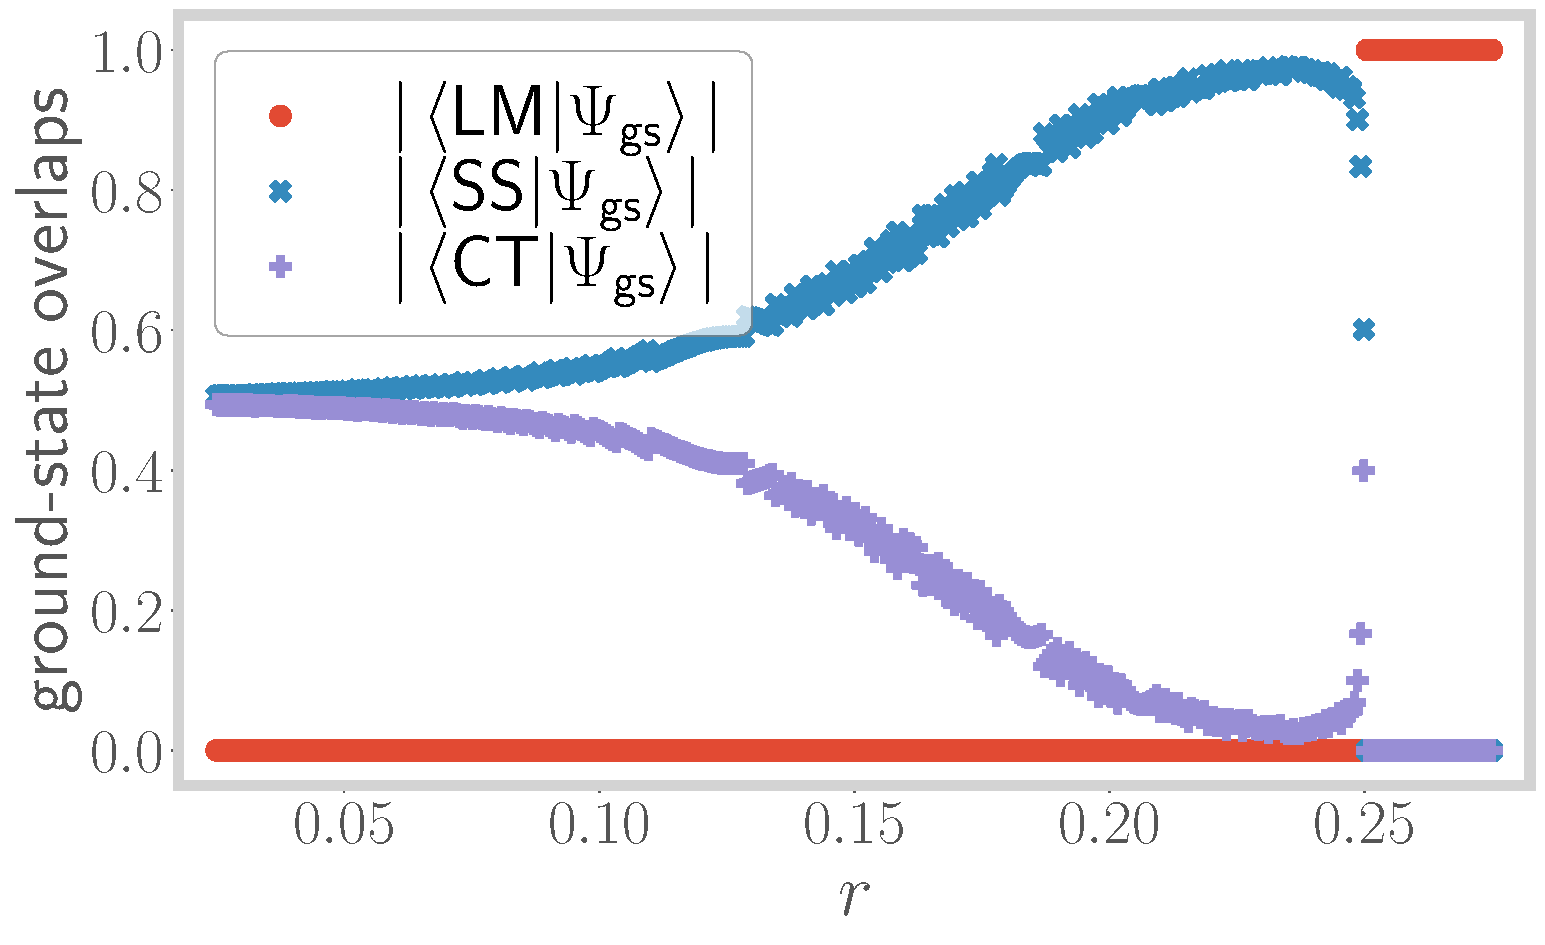
\includegraphics[width=0.5\textwidth]{../figures/corrs_gs.pdf}
\caption{Overlap of the RG fixed point ground state \(\ket{\Psi}_\text{gs}\) with the spin singlet state \(\ket{\text{ss}}\) and the charge triplet state \(\ket{\text{ct}}\), for a range of values of the transition tuning ratio \(r\). Beyond the critical point \(r > 0.25\), both these overlaps vanish.}
	\label{overlaps}
\end{figure}


\section{Descriptors of the transition}

In this section, we will discuss various diagnostics that track the impurity phase transition; these diagnostics or probes will also answer other interesting questions:
\begin{itemize}
	\item[1.] What are the fluctuations that force the transition?
	\item[2.] How do entanglement measures behave across the transition?
	\item[3.] How does the Kondo screening cloud~\cite{}[CITE] respond as the system is driven critical?
\end{itemize}

\subsection{Impurity spectral function}

One of the most obvious indicators of the transition is the appearance of a gap in the spectral function \(A_d(\omega)\) of the impurity. In the AIM, the spectral function \(A_d\) has a single peak structure for small \(U\), and two additional side peaks appear at large \(U\). Although the central peak keeps getting sharper as \(U\) is increased, it never disappears, simply because the impurity is always able to bind with the zeroth site and form a single site; indeed, it is the local Fermi liquid excitations that appear on top of this singlet ground state that gives rise to the central Abrikosov-Suhl resonance in the spectral function~\cite{}[lots of CITE here].

In contrast, the GAIM shows the appearance of a gap as \(r\) crosses \(1/4\) (see Fig.~\ref{spec-func}); the three-peak form survives only up to the critical point. The spectral functions are calculated by numerically diagonalising the effective Hamiltonian obtained from the RG. In the unscreened regime \(r > 0.25\), the impurity spectral function has a two peaks at energies \(\omega = \pm U/2\) corresponding to the fluctuations that create a particle or a hole on the impurity site. The appearance of the gap shows that exactly at \(r=0.25\), the zero-energy pole in the impurity Greens function \(G_d(\omega)\) gets replaced by a zero; this is accompanied by a zero energy divergence in the impurity self-energy \(\Sigma_d = 1/G_d^{(0)}(\omega) - 1/G_d(\omega)\). The expression of the self-energy follows from Dyson's equation, \(G_d^{(0)}(\omega)\) being the self-energy of the impurity at \(U=0\).

\begin{figure}[!htb]
	\centering
	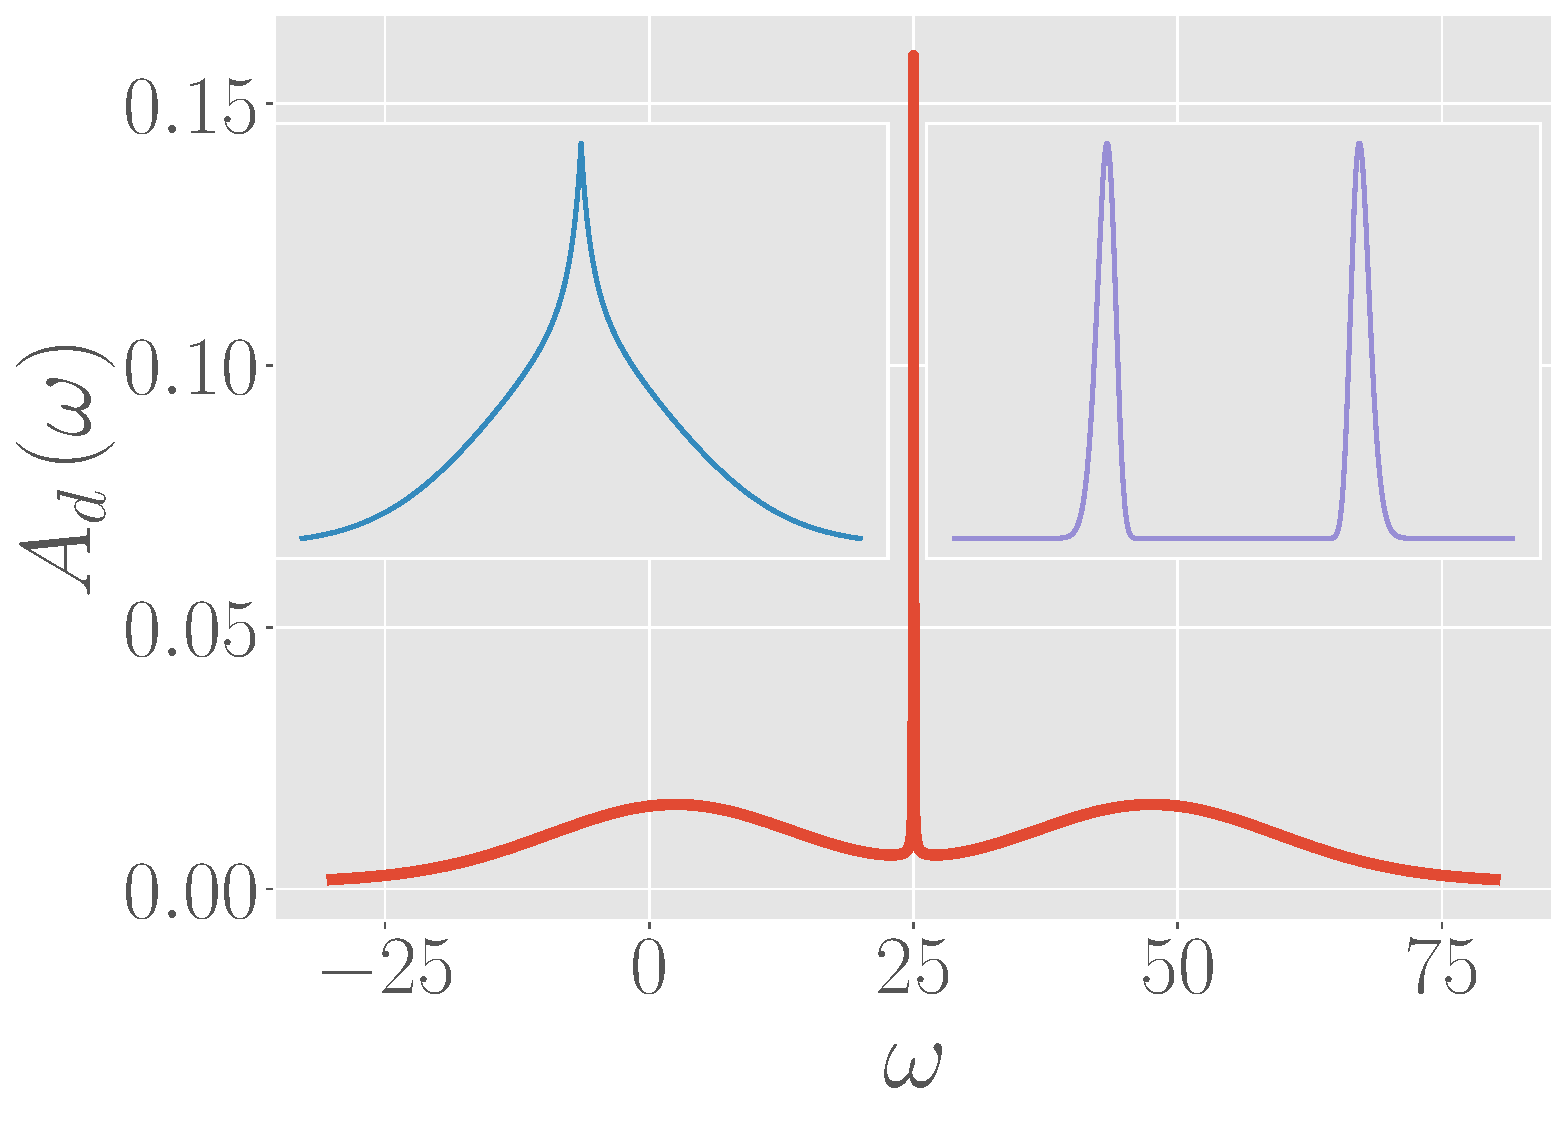
\includegraphics[width=0.5\textwidth]{../figures/Add.pdf}
	\caption{Impurity spectral function \(A_d(\omega)\) at three values of the ratio \(r\). The central large plot is exactly at the critical point \(r=0.25\), the left (blue) inset is at \(r < 0.25\) and the right (violet) inset is at \(r > 0.25\).}
	\label{spec-func}
\end{figure}

\subsection{Using geometric entanglement to track the transition}

The impurity Greens function can be given a spectral representation in terms of the eigenstates \(\left\{\ket{\Psi}_n\right\}\) of the GAIM:
\begin{equation}\begin{aligned}
G_d(\omega) = \sum_n \left[ \frac{|\braket{\Psi_\text{gs} | c_{d\sigma} | \Psi_n}|^2}{\omega + E_\text{gs} - E_n} + \frac{|\braket{\Psi_n | c_{d\sigma} | \Psi_\text{gs}}|^2}{\omega - E_\text{gs} + E_n}\right] 
\end{aligned}\end{equation}
We will now introduce a complete basis into the expression. The basis will be the set of eigenstates of the Hamiltonian  \(H = H_1 + H_2\), where \(H_1\) is the two-site Hamiltonian in eq.~\ref{two-site}, and \(H_2\) is a tight-binding Hamiltonian formed by the remaining sites. Since the Hamiltonians are decoupled, the eigenstates \(\ket{\Psi}_{m,n}\) will be direct product states formed by combining the eigenstates \(\ket{\phi}_m,\ket{\psi}_n\) of the individual Hamiltonians \(H_1\) and \(H_2\) respectively: \(\ket{\Phi}_{m,n} = \ket{\phi}_m\otimes\ket{\psi}_n\). Inserting this basis leads to the expression:
\begin{equation}\begin{aligned}
	\label{summation}
	\ket{\Psi}_\text{gs} = \sum_{m,n} \ket{\Phi}_{m,n} \left(\bra{\phi_{m}}\otimes\bra{\psi_n}\right)\ket{\Psi_\text{gs}}
\end{aligned}\end{equation}
The ground state of \(H_1\) is the spin singlet: \(\ket{\phi}_0 = \ket{\text{ss}}\). We denote the ground state of the tight-binding Hamiltonian \(H_2\) by \(\ket{\psi}_0\). Because of the highly renormalised couplings \(V\) and \(J\), the impurity site is almost maximally entangled with the zeroth site, such that the ground state \(\ket{\Psi}_\text{gs}\) in the \(r < 0.25\) regime can be thought of as a direct product of the two-site ground state, \(c\ket{\text{ss}} + \sqrt{1-c^2}\ket{\text{ct}}\), in direct product with the tight-binding ground state:
\begin{equation}\begin{aligned}
	\ket{\Psi}_\text{gs} \simeq \left(c\ket{\text{ss}} + \sqrt{1-c^2}\ket{\text{ct}}\right)  \otimes \ket{\psi}_0 = \ket{\Phi}_\text{ss} + \ket{\Phi}_\text{ct}
\end{aligned}\end{equation}
where \(\ket{\Phi}_\text{ss(ct)} = \ket{\text{ss}\left( \text{ct} \right)}\otimes\ket{\psi}_0 \).
This suggests that not all terms in the summation of eq.~\ref{summation} contribute; out of all \(\left\{ \ket{\psi}_n \right\} \), only the ground state \(n=0\) contributes, while only \(\ket{ss}\) and \(\ket{ct}\) contribute from the set \(\left\{ \ket{\phi}_m \right\} \). The summation then simplifies to
\begin{equation}\begin{aligned}
	\ket{\Psi}_\text{gs} = \ket{\Phi}_{ss}\braket{\text{ss}|\Psi^{(2)}_\text{gs}} + \ket{\Phi}_{ct}\braket{\text{ct}|\Psi^{(2)}_\text{gs}}~,
\end{aligned}\end{equation}
where \(\ket{\Psi^{(2)}_\text{gs}}\) is the two-site part of the ground state and can be obtained by starting with the full ground state \(\ket{\Psi}_\text{gs}\) and tracing over the other lattice sites of the system.

{\color{blue}We assume that the global phase of the wavefunctions are real}, and since the internal weights of the wavefunctions are real as well, the overlaps \(\braket{\text{ss}|\Psi^{(2)}_\text{gs}},\braket{\text{ct}|\Psi^{(2)}_\text{gs}}\) are also real. We can use these overlaps to define a geometric measure of entanglement:
\begin{equation}\begin{aligned}
	\varepsilon\left(\psi_1,\psi_2\right) = 1 - |\braket{\psi_1 | \psi_2}|^2
\end{aligned}\end{equation}
[CITE]
If \(\ket{\psi_1}\) is thought of as a separable state, then \(\ket{\psi_2}\) should be less entangled if it's overlap with \(\ket{\psi_1}\) is large, which is indeed borne out by the definition.
The overlaps then become \(\braket{\text{ss}|\Psi^{(2)}_\text{gs}} = \sqrt{1 - \varepsilon\left(ss,\Psi^{(2)}_\text{gs}\right)}\), and similarly for the state \(\ket{\text{ct}}\). For brevity, we will use the notation \(\varepsilon_\text{ss} \equiv \varepsilon\left(ss,\Psi^{(2)}_\text{gs}\right), \varepsilon_\text{ct} \equiv \varepsilon\left(ct,\Psi^{(2)}_\text{gs}\right)\). The Greens function can now be written in terms of these measures:
\begin{widetext}
\begin{equation}\begin{aligned}
	G_d(\omega) = \sum_n \left[\left(1 - \varepsilon_\text{ss} \right) \left(\frac{|\braket{\Phi_\text{ss} | c_{d\sigma} | \Psi_n}|^2}{\omega + E_\text{gs} - E_n} + \frac{|\braket{\Psi_n | c_{d\sigma} | \Phi_\text{ss}}|^2}{\omega - E_\text{gs} + E_n}\right) + \left(1 - \varepsilon_\text{ct} \right) \left(\frac{|\braket{\Phi_\text{ct} | c_{d\sigma} | \Psi_n}|^2}{\omega + E_\text{gs} - E_n} + \frac{|\braket{\Psi_n | c_{d\sigma} | \Phi_\text{ct}}|^2}{\omega - E_\text{gs} + E_n}\right)\right.\\
	+ \left. \sqrt{\left(1 - \varepsilon_\text{ss} \right)}\sqrt{\left(1 - \varepsilon_\text{ct} \right)} \left(\frac{\braket{\Phi_\text{ss} | c_{d\sigma} | \Psi_n}\braket{\Psi_n | c^\dagger_{d\sigma} | \Phi_\text{ct}} + \text{h.c.}}{\omega + E_\text{gs} - E_n} + \frac{\braket{\Phi_\text{ct} | c_{d\sigma} | \Psi_n}\braket{\Psi_n | c^\dagger_{d\sigma} | \Phi_\text{ss}} + \text{h.c.}}{\omega - E_\text{gs} + E_n}\right)\right]
\end{aligned}\end{equation}
\end{widetext}

\begin{figure}[htpb]
	\centering
	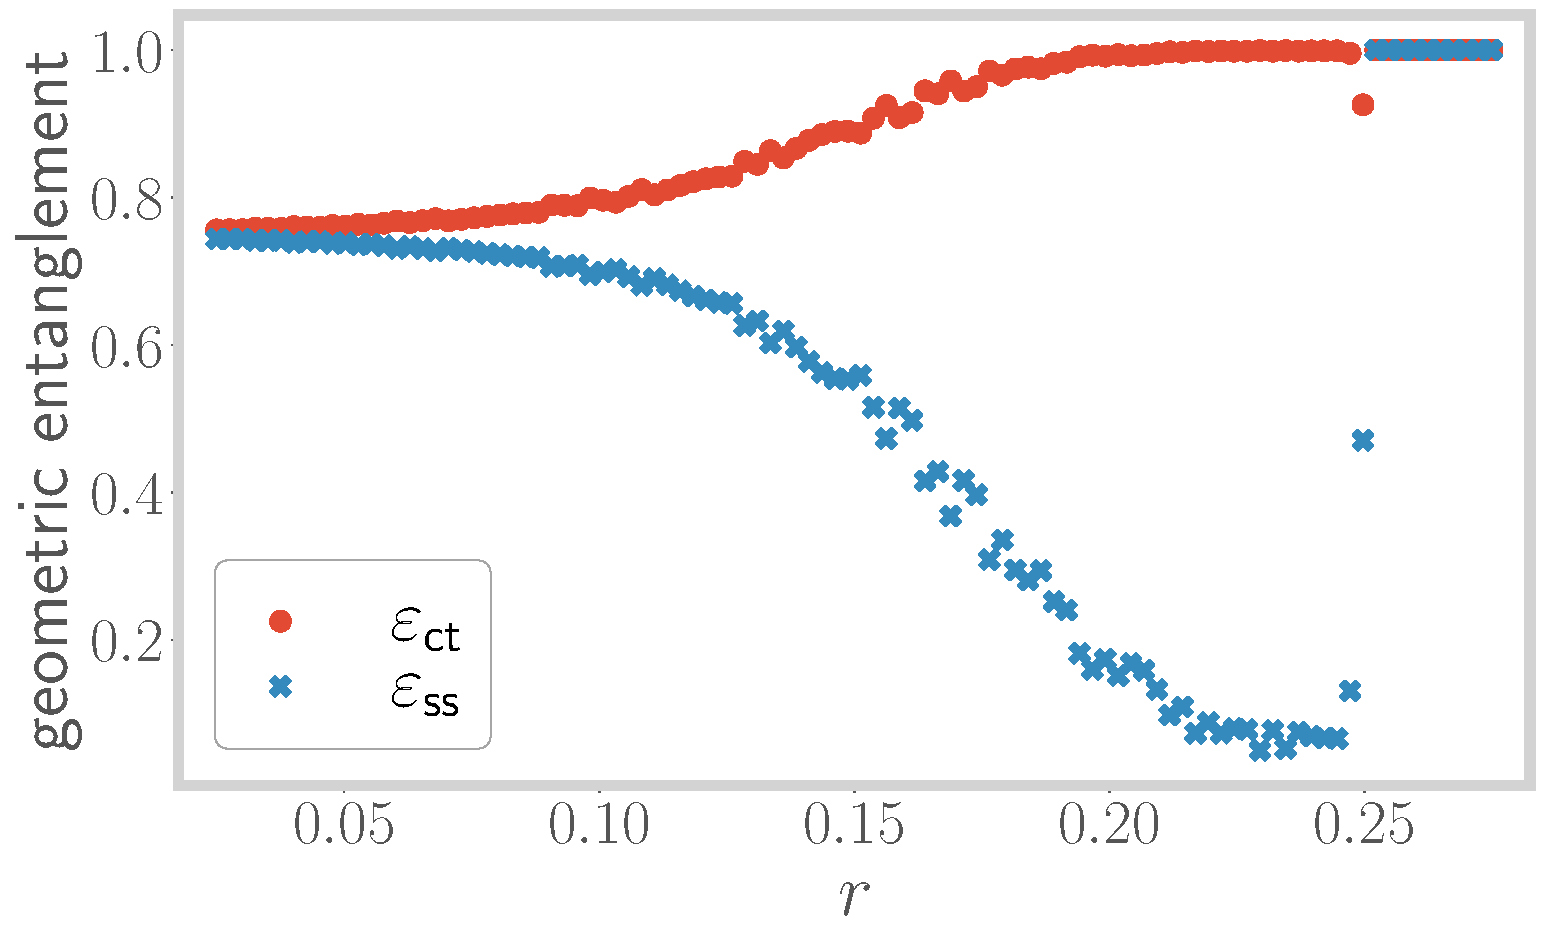
\includegraphics[width=0.5\textwidth]{../figures/entanglement.pdf}
	\caption{Variation of \(\sqrt{\left(1 - \varepsilon_\text{ss} \right)}\sqrt{\left(1 - \varepsilon_\text{ct} \right)}\) as \(r\) is increased towards the critical value 0.25. Inset shows the variation of the individual measures \(\varepsilon_\text{ss},\varepsilon_\text{ct}\).}
	\label{entng}
\end{figure}

This expression is interesting because it relates the Greens function (measurable when converted into a spectral function) to measures of entanglement.
These measures have been plotted up to the critical point in Fig.~\ref{entng}.
While \(\varepsilon_\text{ss},\varepsilon_\text{ct}\) (plotted in the inset) are very similar to the overlaps plotted in Fig.~\ref{overlaps}, the cross-term \(\sqrt{\left(1 - \varepsilon_\text{ss} \right)}\sqrt{\left(1 - \varepsilon_\text{ct} \right)}\) plotted in the main figure has an overall monotonic incremental behaviour towards the transition.
We can now use the knowledge of the behaviour of these measures to make some statements about the nature of the transition from the Greens function.
Since \(\varepsilon_\text{ss}\) increases towards the transition, we find that the first major term in the Greens function decreases; this shows that scattering within the spin sector loses weight.
On the other hand, since \(\varepsilon_\text{ct}\) decreases, the second major term in \(G_d\) increases, reflecting the growth in the participation of the charge sector in the scattering processes.
The final major term also increases, due to the monotonic growth of \(\sqrt{\left(1 - \varepsilon_\text{ss} \right)}\sqrt{\left(1 - \varepsilon_\text{ct} \right)}\), showing that there is a continual increase in the {\it mixing of the spin and charge sectors}.

\subsection{Presence of sub-dominant pair fluctuations}

\begin{figure}
	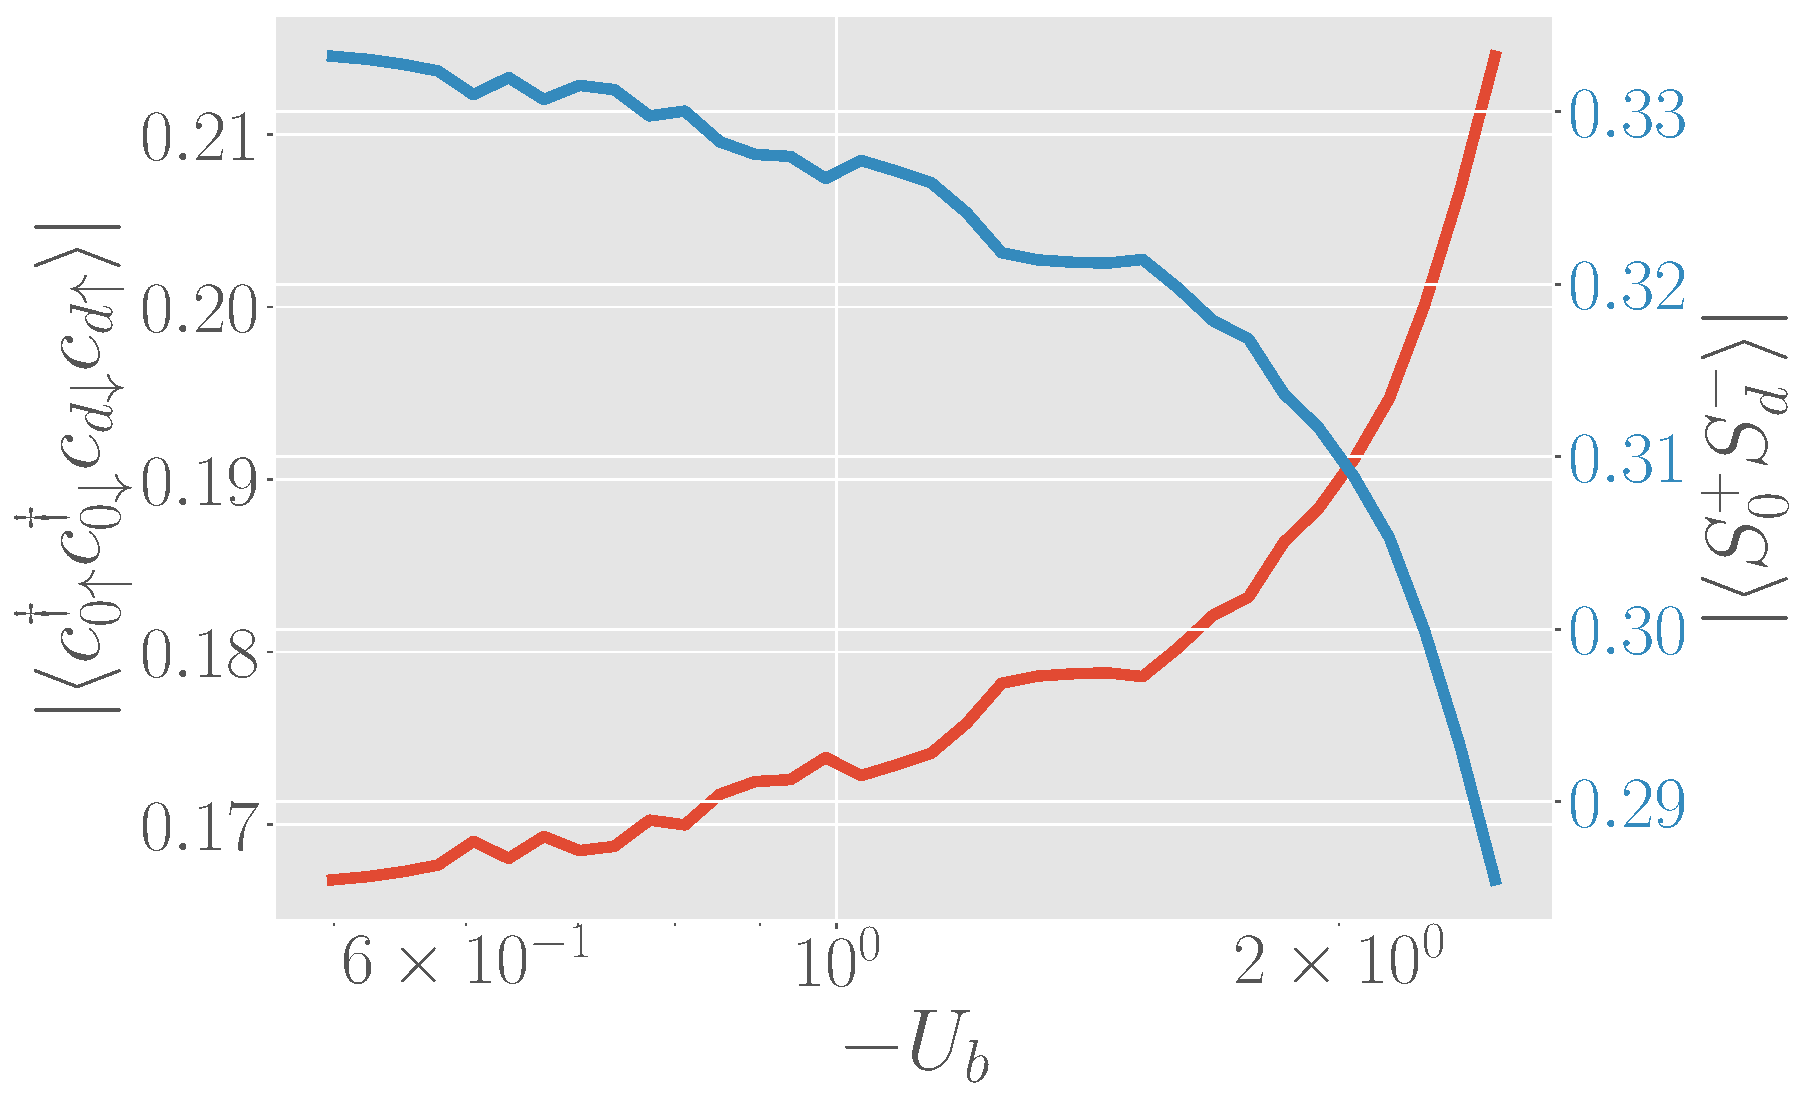
\includegraphics[width=0.49\textwidth]{../figures/odlro.pdf}
	\caption{Growth of pair fluctuations \(p^\dagger_d p_0\) between the impurity and the zeroth site towards the critical point, \(p^\dagger=c^\dagger_\uparrow c^\dagger_\downarrow\) being the local pair creation operator. This comes at the cost of the spin-flip fluctuations \(S_d^+ s_0^- + \text{h.c.}\), which decrease towards the transition.}
	\label{pair_fluc}
\end{figure}

\subsection{Mutual information and entanglement entropy in the ground state: fate of the Kondo cloud}
Since the system has to undergo a phase transition into an unscreened phase for \(r > 0.25\), it is clear that the Kondo screening cloud must disappear. Indeed, this is captured by various entanglement measures like mutual information and entanglement entropy. The entanglement entropy of subsystem \(A\) with the rest is defined as
\begin{equation}\begin{aligned}
	S(A) = \text{Tr}\left[\rho_A \ln \rho_A\right]
\end{aligned}\end{equation}
where \(\rho_A\) is the reduced density matrix obtained by tracing the full density matrix \(\rho = \ket{\Psi}_\text{gs} \bra{\Psi}_\text{gs}\) over all subsystems apart from \(A\). The mutual information between two subsystems \(A\) and \(B\) is defined as
\begin{equation}\begin{aligned}
	I(A:B) = S(A) + S(B) - S(A \cup B)
\end{aligned}\end{equation}
where \(S(A \cup B)\) is the entanglement entropy of \(A\) and \(B\) with the rest. I(A:B) represents the amount of information that can be gained about \(B\) on measuring \(A\), or vice-versa. If the ground state \(\ket{\Psi}_\text{gs}\) is a separable state where \(A\) is a disentangled from the rest, then its entanglement entropy \(S(A)\) will be \(0\). On the other hand, if the ground state cannot be written in separable form, \(S(A)\) becomes non-zero, and the maximum value it can take is \(\ln d\), where \(d\) is the dimension of the Hilbert space of \(A\). 

In the AIM or the Kondo model ground state, the impurity forms a maximally entangled singlet with the zeroth site. This in turn leads to entanglement in \(k-\)space between the conduction electrons that screen the impurity and form the Kondo cloud~\cite{anirban_kondo}. 

\begin{figure}[!htb]
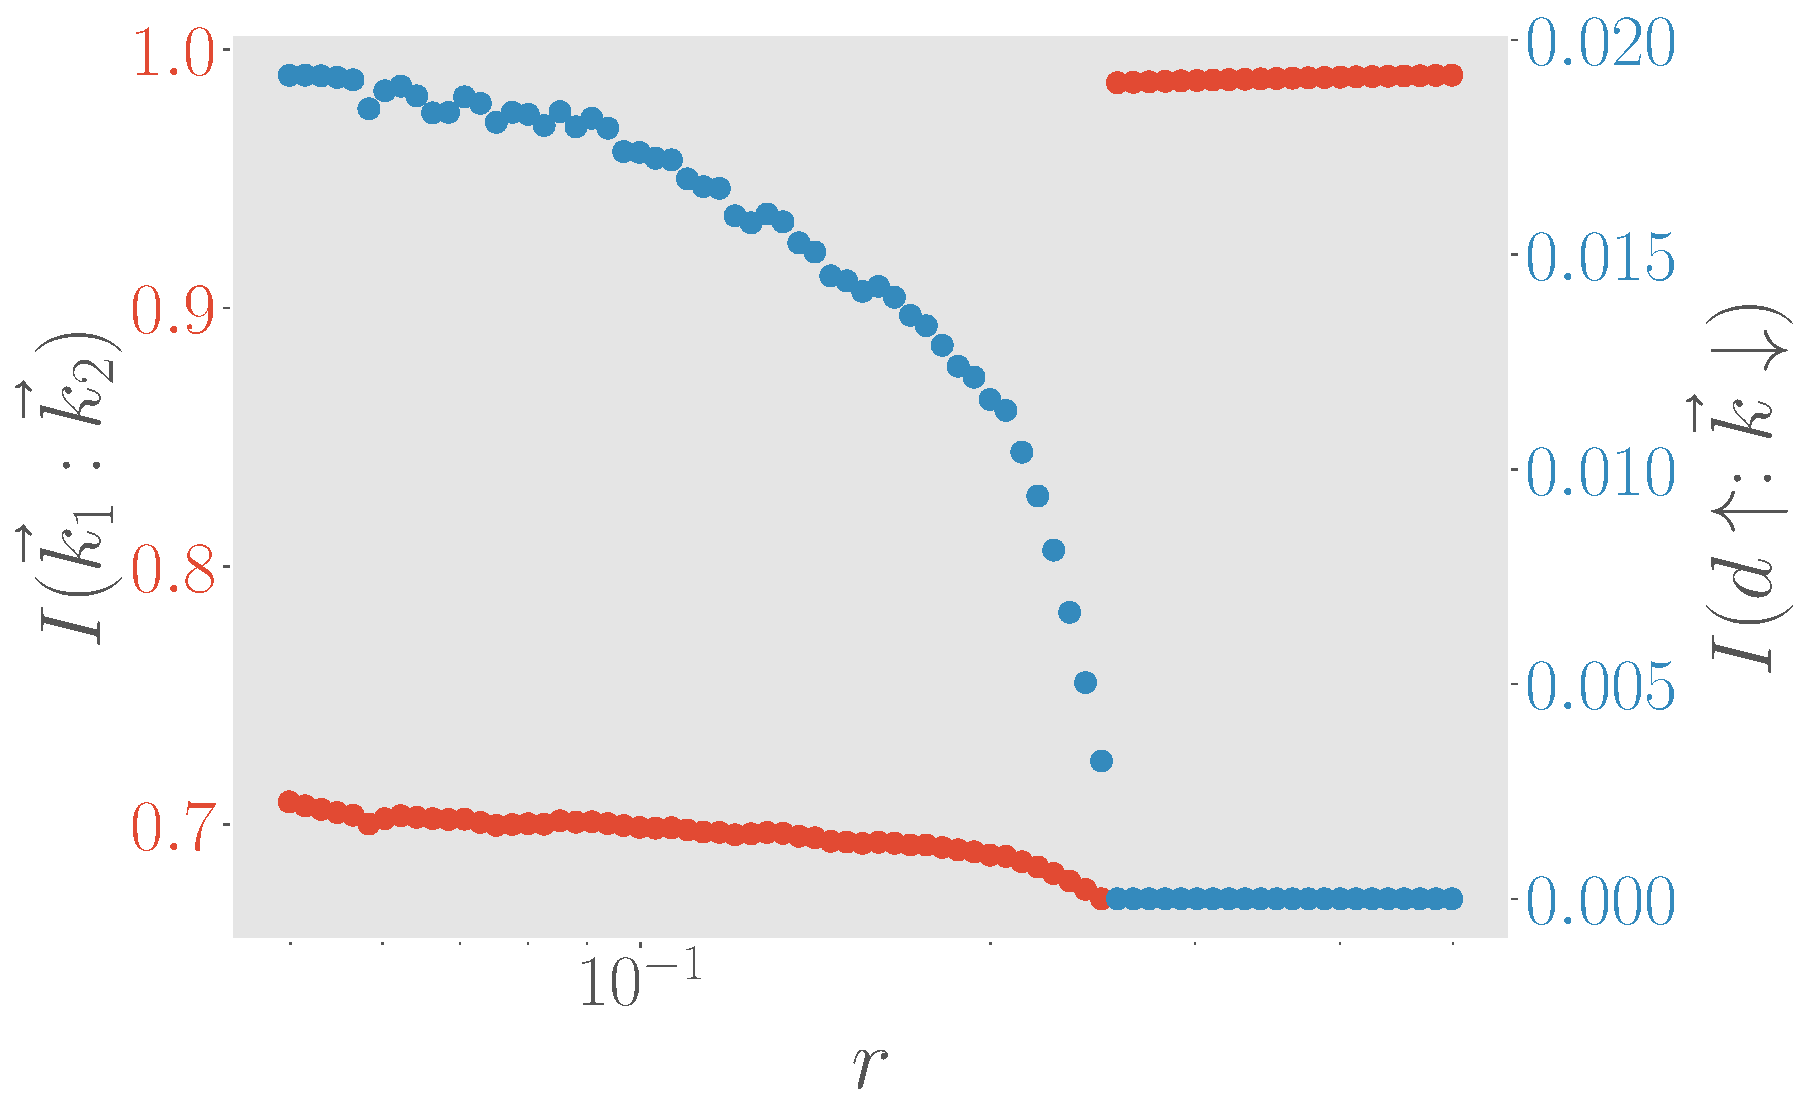
\includegraphics[width=0.49\textwidth]{../figures/I_k.pdf}
\caption{caption}
\end{figure}
\begin{figure}[!htb]
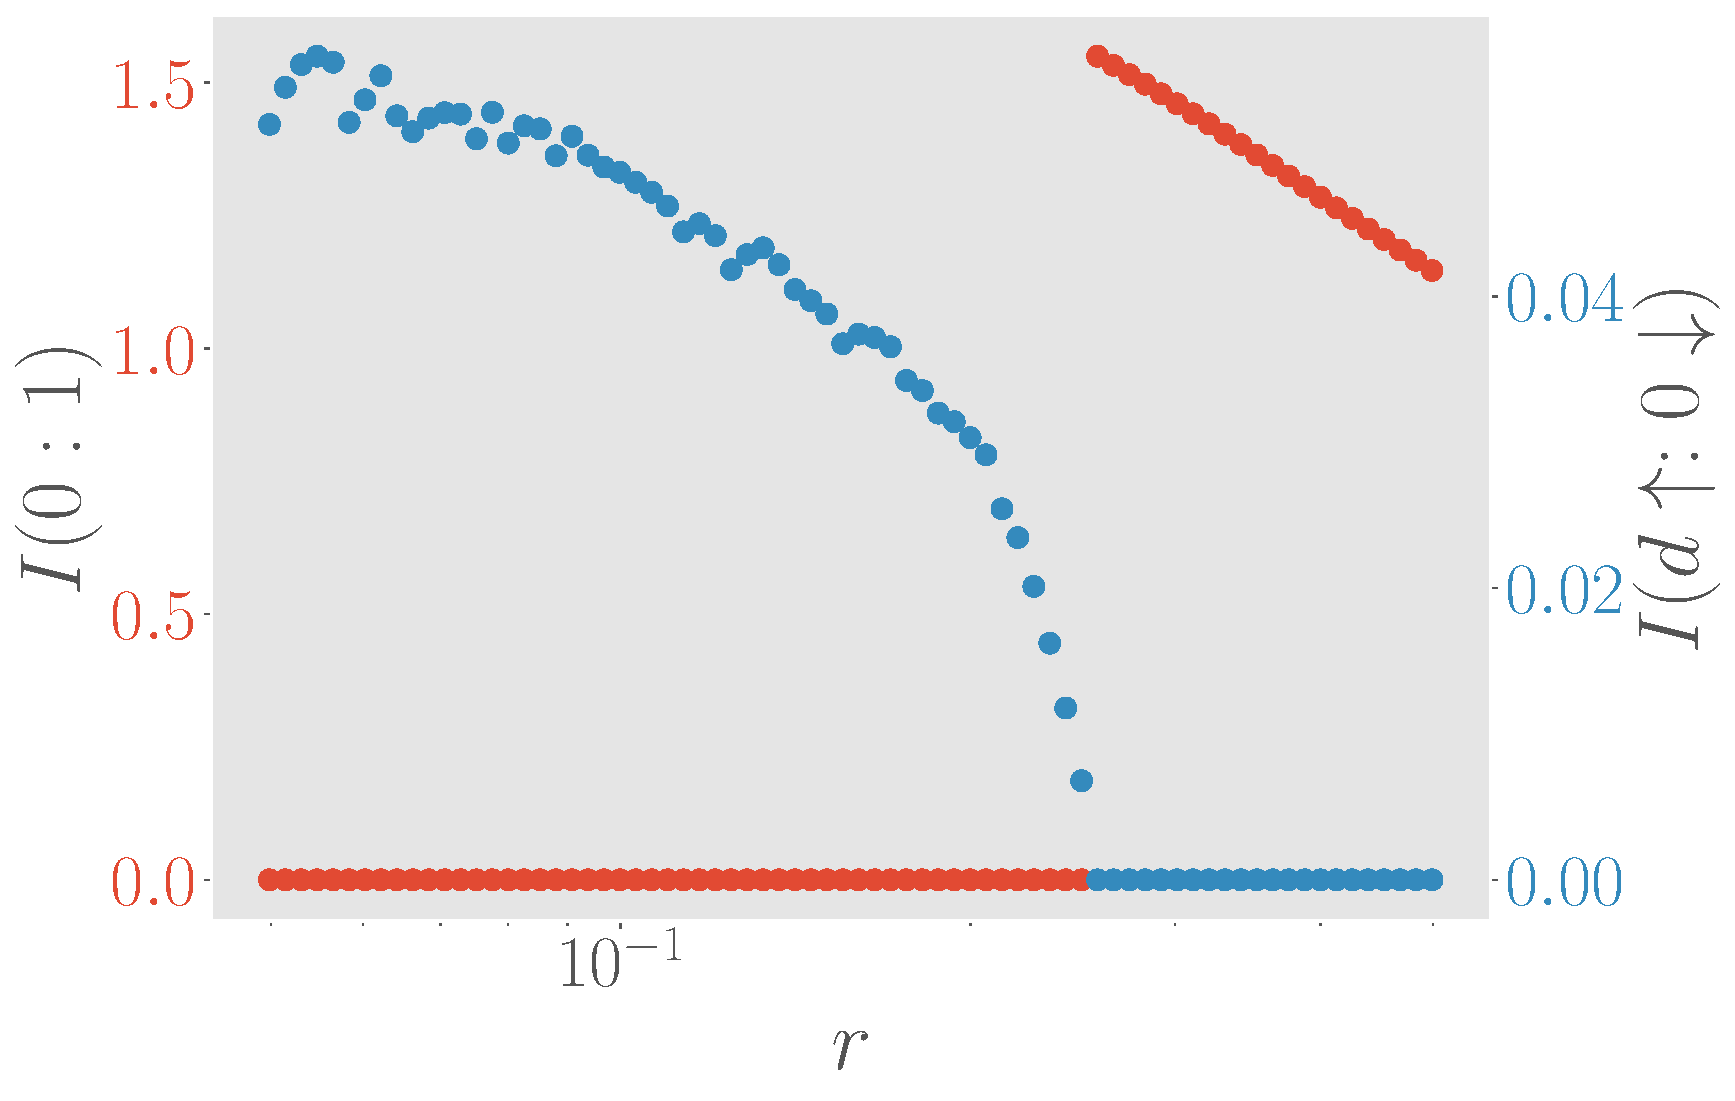
\includegraphics[width=0.49\textwidth]{../figures/I_r.pdf}
\caption{caption}
\end{figure}
\begin{figure}[!htb]
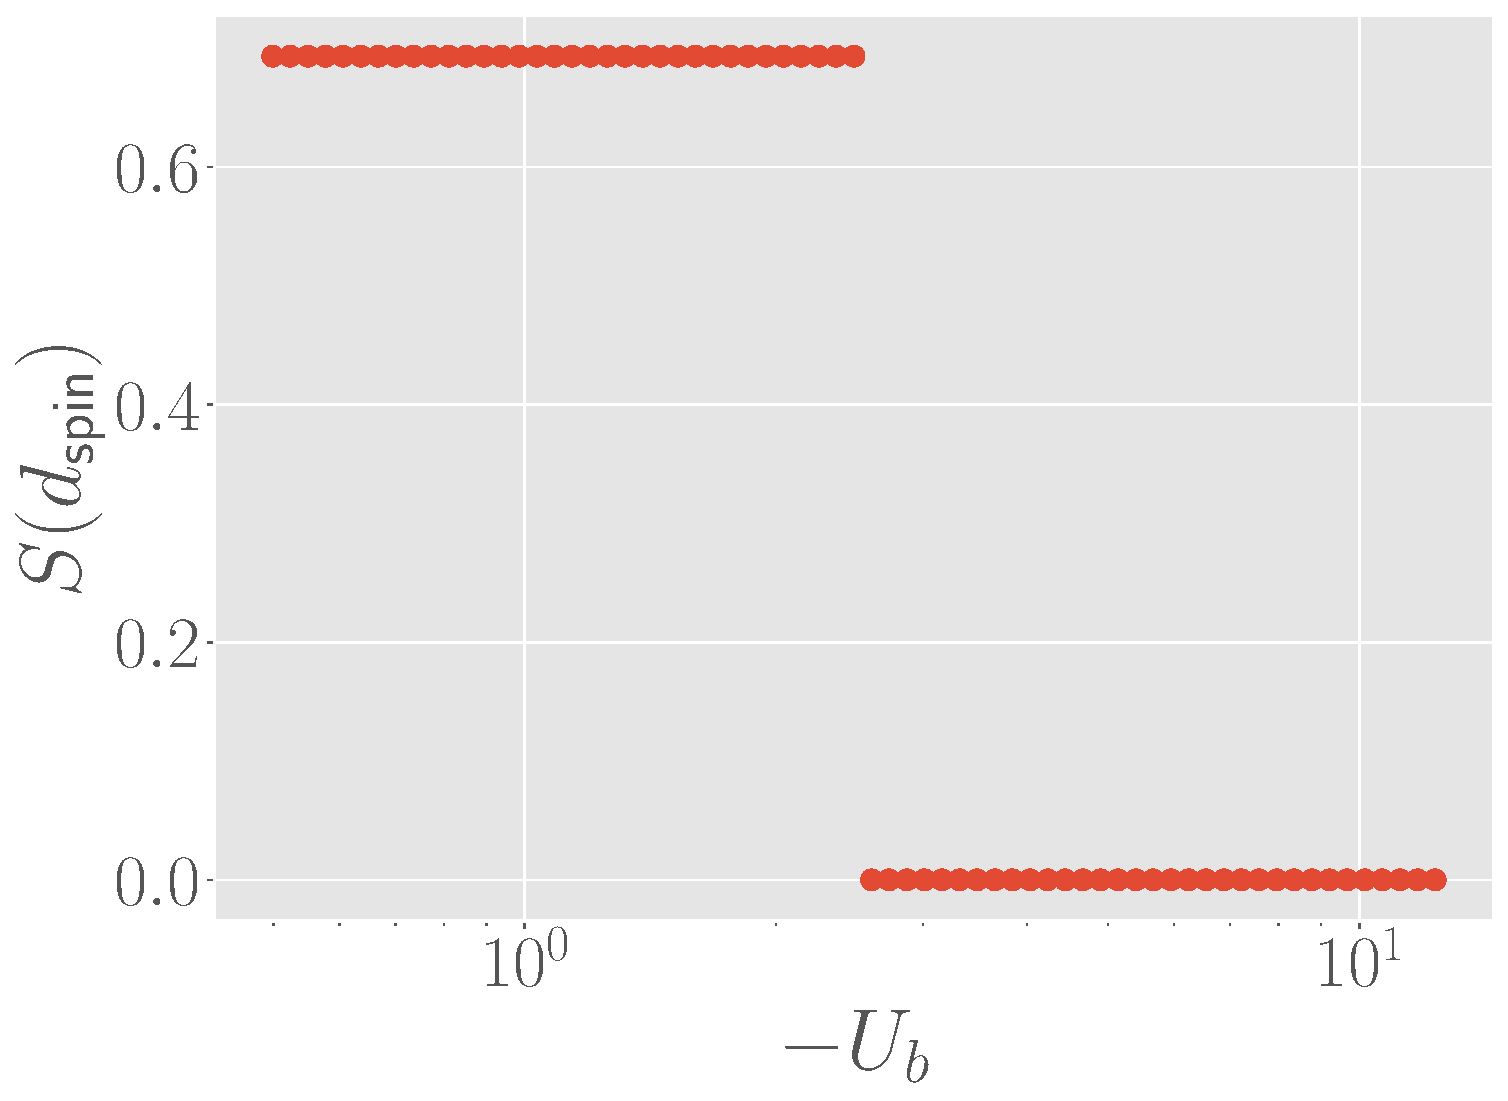
\includegraphics[width=0.49\textwidth]{../figures/S_imp.pdf}
\caption{caption}
\end{figure}

\section{Conclusions}
CC
Lorem ipsum dolor sit amet, consectetur adipiscing elit, sed do eiusmod tempor incididunt ut labore et dolore magna aliqua. Ut enim ad minim veniam, quis nostrud exercitation ullamco laboris nisi ut aliquip ex ea commodo consequat. Duis aute irure dolor in reprehenderit in voluptate velit esse cillum dolore eu fugiat nulla pariatur. Excepteur sint occaecat cupidatat non proident, sunt in culpa qui officia deserunt mollit anim id est laborumLorem ipsum dolor sit amet, consectetur adipiscing elit, sed do eiusmod tempor incididunt ut labore et dolore magna aliqua. Ut enim ad minim veniam, quis nostrud exercitation ullamco laboris nisi ut aliquip ex ea commodo consequat. Duis aute irure dolor in reprehenderit in voluptate velit esse cillum dolore eu fugiat nulla pariatur. Excepteur sint occaecat cupidatat non proident, sunt in culpa qui officia deserunt mollit anim id est laborumLorem ipsum dolor sit amet, consectetur adipiscing elit, sed do eiusmod tempor incididunt ut labore et dolore magna aliqua. Ut enim ad minim veniam, quis nostrud exercitation ullamco laboris nisi ut aliquip ex ea commodo consequat. Duis aute irure dolor in reprehenderit in voluptate velit esse cillum dolore eu fugiat nulla pariatur. Excepteur sint occaecat cupidatat non proident, sunt in culpa qui officia deserunt mollit anim id est laborum
Lorem ipsum dolor sit amet, consectetur adipiscing elit, sed do eiusmod tempor incididunt ut labore et dolore magna aliqua. Ut enim ad minim veniam, quis nostrud exercitation ullamco laboris nisi ut aliquip ex ea commodo consequat. Duis aute irure dolor in reprehenderit in voluptate velit esse cillum dolore eu fugiat nulla pariatur. Excepteur sint occaecat cupidatat non proident, sunt in culpa qui officia deserunt mollit anim id est laborumLorem ipsum dolor sit amet, consectetur adipiscing elit, sed do eiusmod tempor incididunt ut labore et dolore magna aliqua. Ut enim ad minim veniam, quis nostrud exercitation ullamco laboris nisi ut aliquip ex ea commodo consequat. Duis aute irure dolor in reprehenderit in voluptate velit esse cillum dolore eu fugiat nulla pariatur. Excepteur sint occaecat cupidatat non proident, sunt in culpa qui officia deserunt mollit anim id est laborumLorem ipsum dolor sit amet, consectetur adipiscing elit, sed do eiusmod tempor incididunt ut labore et dolore magna aliqua. Ut enim ad minim veniam, quis nostrud exercitation ullamco laboris nisi ut aliquip ex ea commodo consequat. Duis aute irure dolor in reprehenderit in voluptate velit esse cillum dolore eu fugiat nulla pariatur. Excepteur sint occaecat cupidatat non proident, sunt in culpa qui officia deserunt mollit anim id est laborum
Lorem ipsum dolor sit amet, consectetur adipiscing elit, sed do eiusmod tempor incididunt ut labore et dolore magna aliqua. Ut enim ad minim veniam, quis nostrud exercitation ullamco laboris nisi ut aliquip ex ea commodo consequat. Duis aute irure dolor in reprehenderit in voluptate velit esse cillum dolore eu fugiat nulla pariatur. Excepteur sint occaecat cupidatat non proident, sunt in culpa qui officia deserunt mollit anim id est laborumLorem ipsum dolor sit amet, consectetur adipiscing elit, sed do eiusmod tempor incididunt ut labore et dolore magna aliqua. Ut enim ad minim veniam, quis nostrud exercitation ullamco laboris nisi ut aliquip ex ea commodo consequat. Duis aute irure dolor in reprehenderit in voluptate velit esse cillum dolore eu fugiat nulla pariatur. Excepteur sint occaecat cupidatat non proident, sunt in culpa qui officia deserunt mollit anim id est laborumLorem ipsum dolor sit amet, consectetur adipiscing elit, sed do eiusmod tempor incididunt ut labore et dolore magna aliqua. Ut enim ad minim veniam, quis nostrud exercitation ullamco laboris nisi ut aliquip ex ea commodo consequat. Duis aute irure dolor in reprehenderit in voluptate velit esse cillum dolore eu fugiat nulla pariatur. Excepteur sint occaecat cupidatat non proident, sunt in culpa qui officia deserunt mollit anim id est laborum
Lorem ipsum dolor sit amet, consectetur adipiscing elit, sed do eiusmod tempor incididunt ut labore et dolore magna aliqua. Ut enim ad minim veniam, quis nostrud exercitation ullamco laboris nisi ut aliquip ex ea commodo consequat. Duis aute irure dolor in reprehenderit in voluptate velit esse cillum dolore eu fugiat nulla pariatur. Excepteur sint occaecat cupidatat non proident, sunt in culpa qui officia deserunt mollit anim id est laborumLorem ipsum dolor sit amet, consectetur adipiscing elit, sed do eiusmod tempor incididunt ut labore et dolore magna aliqua. Ut enim ad minim veniam, quis nostrud exercitation ullamco laboris nisi ut aliquip ex ea commodo consequat. Duis aute irure dolor in reprehenderit in voluptate velit esse cillum dolore eu fugiat nulla pariatur. Excepteur sint occaecat cupidatat non proident, sunt in culpa qui officia deserunt mollit anim id est laborumLorem ipsum dolor sit amet, consectetur adipiscing elit, sed do eiusmod tempor incididunt ut labore et dolore magna aliqua. Ut enim ad minim veniam, quis nostrud exercitation ullamco laboris nisi ut aliquip ex ea commodo consequat. Duis aute irure dolor in reprehenderit in voluptate velit esse cillum dolore eu fugiat nulla pariatur. Excepteur sint occaecat cupidatat non proident, sunt in culpa qui officia deserunt mollit anim id est laborum

\begin{itemize}
	\item discuss why the model is minimal
\end{itemize}

\acknowledgments
Abhirup Mukherjee thanks IISER Kolkata for funding through a research fellowship. S. Lal thanks the SERB, Govt. of India for funding through MATRICS grant MTR/2021/000141 and Core Research Grant CRG/2021/000852.

\appendix*

\begin{widetext}
\section{Derivation of RG equations for the generalised Anderson impurity model}

\subsection{Renormalisation of the impurity energy \(\epsilon_d\)}
The coupling \(\epsilon_d\) is renormalised by three kinds of vertices: \(V^2\), \(J^2\) and \(K^2\). We will consider these processes one after another. We define \(n_j\) as the number of states being decoupled on each side of the Fermi surface, at the \(j^\text{th}\) RG step. In order to treat both spin and isospin exchanges democratically, we take \(\ket{\Psi}_i = \frac{1}{2}\left(\ket{0} + \ket{q\uparrow} + \ket{q\downarrow} + \ket{q\uparrow, q\downarrow}\right) \) as the \textit{initial} state for the scattering processes. The intermediate states \(\ket{\Psi}_\text{int}\) in the particle sector \(\left(c_{q\beta}\ket{\Psi}_i\right)\) and hole sector \(\left(c^\dagger_{q\beta}\ket{\Psi}_i\right)\) will then have both spin and isospin excitations which can couple with the corresponding impurity degree of freedom. We will assume that states  \(q > k_F~\left(\epsilon_q > 0\right) \) above the Fermi surface can have only particle excitations and states below the Fermi surface can only have hole excitations. The kinetic energy part \(\epsilon_q \tau_{q\beta}\) of \(H_D\) for \(\ket{\Psi}_i\) is then zero, whereas it is always \(D/2\) for \(\ket{\Psi}_\text{int}\). To demonstrate this for a typical \(q < k_F\), the hole excitation is \(c_{q \uparrow}\ket{\Psi}_i = \frac{1}{\sqrt 2}\left(\ket{0} + \ket{q \downarrow}\right)\). This has an isospin term in the form of the \textit{holon} and a spin term in the form of the down state. Since \(\tau_{q \uparrow} = -\frac{1}{2}\) in the excited state, the kinetic energy for \(\ket{\Psi}_\text{int}\) is \(\epsilon_q \tau_{q \uparrow} = \left(-D\right)\times\left(-\frac{1}{2}\right) = D/2\).

The renormalisation arising from the first kind of terms, in the particle sector, is
\begin{equation}\begin{aligned}
	\sum_{q\beta}c^\dagger_{q\beta}c_{d\beta}\frac{V^2}{\omega - H_D}c^\dagger_{d\beta}c_{q\beta} = \sum_{q\beta}V^2 \hat n_{q\beta} \left( 1 - \hat n_{d\beta} \right)\left( \frac{1-\hat n_{d \overline\beta }}{\omega - E_0} + \frac{\hat n_{d \overline\beta}}{\omega^\prime - E_1}\right) = V^2 n_j\sum_{\beta}\left( 1 - \hat n_{d\beta} \right)\left( \frac{1-\hat n_{d \overline\beta }}{\omega_0 - E_0} + \frac{\hat n_{d \overline\beta}}{\omega_1 - E_1}\right)
\end{aligned}\end{equation}
\(q\) runs over the momentum states that are being decoupled at this RG step: \(|q| = \Lambda_j\). \(E_{1,0}\) are the diagonal parts of the Hamiltonian at \(\hat n_{d\overline \beta}=1,0\) respectively. We have \(\hat n_{d\beta}=1\) in the intermediate state because of the \(c^\dagger_{d\beta}\) in front of the Greens function. Applying \(c_{q\beta}\) on the initial state \(\ket{\Psi}_i\) leaves us with \(C^z_q = - \frac{1}{2}\) and \(s^z_q = \frac{1}{2}\overline\beta\). We also know that
\begin{equation}\begin{aligned}
	\hat n_{d\beta}=1,
	\begin{cases}
		\hat n_{d\overline\beta}=0 &\implies S_d^z = \frac{1}{2}\beta, C_d^z = 0, \epsilon_d\left(\hat n_{d\uparrow} - \hat n_{d \downarrow}\right)^2 = \epsilon_d\\	
		\hat n_{d\overline\beta}=1 &\implies S_d^z = 0, C_d^z = \frac{1}{2}, \epsilon_d\left(\hat n_{d\uparrow} - \hat n_{d \downarrow}\right)^2 = 0
	\end{cases}
\end{aligned}\end{equation}
Combining all this, we can write \(E_1 = \frac{D}{2} - \frac{K}{4}\) and \(E_0 = \frac{D}{2} + \epsilon_d - \frac{J}{4}\). In order to relate \(\omega_0\) with \(\omega_1\) with the common fluctuation scale \(\omega\) for the conduction electrons, we will replace these quantum fluctuation scales by the current renormalised values of the single-particle self-energy for the initial state from which we started scattering. For \(\hat n_{d\overline\beta}=0\), there is no additional self-energy because the impurity does not have any spin: \(\omega_0 = \omega\). For \(\hat n_{d\overline\beta} = 1\), we have an additional self-energy of \(\epsilon_d\) arising from the correlation on the impurity: \(\omega_1 = \omega + \epsilon_d\).
Substituting the values of \(E_{0,1}\) and \(\omega_{0,1}\), we get
\begin{equation}\begin{aligned}
	\label{ren_ed_Vp}
	V^2 n_j\sum_{\beta}\left( 1 - \hat n_{d\beta} \right)\left( \frac{1-\hat n_{d \overline\beta }}{\omega - \frac{D}{2} - \epsilon_d + \frac{J}{4}} + \frac{\hat n_{d \overline\beta}}{\omega - \frac{D}{2} + \epsilon_d + \frac{K}{4}}\right)
\end{aligned}\end{equation}
Performing a similar calculation for the hole sector gives the contribution:
\begin{equation}\begin{aligned}
	\label{ren_ed_Vh}
	V^2 n_j\sum_{\beta}\hat n_{d\beta}\left( \frac{1-\hat n_{d \overline\beta }}{\omega - \frac{D}{2} + \epsilon_d + \frac{K}{4}} + \frac{\hat n_{d \overline\beta}}{\omega - \frac{D}{2} - \epsilon_d + \frac{J}{4}}\right)
\end{aligned}\end{equation}
We now come to the second type of terms: spin-spin. We first look at the particle sector:
\begin{equation}\begin{aligned}
	\label{ren_ed_Jpp}
	\frac{J^2}{4}\sum_{q\beta}c^\dagger_{d\overline\beta}c_{d\beta}c^\dagger_{q\beta}c_{-q\overline\beta} \frac{1}{\omega - H_D}c^\dagger_{d\beta}c_{d\overline\beta}c^\dagger_{q\overline\beta}c_{q\beta} = \frac{J^2}{4} n_j\frac{1}{\omega - \frac{D}{2} + \frac{J}{4}} \sum_{\beta}\hat n_{d\overline\beta}\left( 1 - \hat n_{d\beta} \right)
\end{aligned}\end{equation}
The diagonal part in the denominator was simple to deduce in this case, because the nature of the scattering requires the spins \(S_d^z\) and \(\frac{\beta}{2}\left(\hat n_{q\beta} - \hat n_{q \overline\beta}\right)\) to be anti-parallel. This ensures that the intermediate state has an energy of \(E = \frac{D}{2} + \epsilon_d - \frac{J}{4}\), and the quantum fluctuation scale is \(\omega^\prime = \omega + \epsilon_d\), such that \(\omega^\prime - E = \omega - \frac{D}{2} + \frac{J}{4}\). In the hole sector, we have
\begin{equation}\begin{aligned}
	\label{ren_ed_Jph}
	\frac{J^2}{4} n_j\frac{1}{\omega - \frac{D}{2} + \frac{J}{4}} \sum_{\beta}\hat n_{d\beta}\left( 1 - \hat n_{d\overline\beta} \right)
\end{aligned}\end{equation}
The final kind of scattering is the \(K^2\) type. Similar to the \(J^2\) term, we get the following contribution:
\begin{equation}\begin{aligned}
	\label{ren_ed_Kpp}
	\frac{K^2}{4}\sum_{q\beta}c^\dagger_{q\beta}c^\dagger_{q\overline\beta}c_{d\overline\beta}c_{d\beta} \frac{1}{\omega - H_D}c^\dagger_{d\beta}c^\dagger_{d\overline\beta}c_{q\overline\beta}c_{q\beta} = \frac{K^2}{2} n_j\frac{1}{\omega - \frac{D}{2} + \frac{K}{4}} \left(1 - \hat n_{d \uparrow}\right) \left( 1 - \hat n_{d \downarrow} \right)
\end{aligned}\end{equation}
in the particle sector. This is again because \(E = \frac{D}{2} - \frac{K}{4}\) in the intermediate state and \(\omega^\prime = \omega\). In the hole sector, we get
\begin{equation}\begin{aligned}
	\label{ren_ed_Kph}
	\frac{K^2}{2} n_j\frac{1}{\omega - \frac{D}{2} + \frac{K}{4}} \hat n_{d\uparrow}\hat n_{d \downarrow}~.
\end{aligned}\end{equation}

We now have all possible renormalisation to the impurity energy \(\epsilon_d\). To actually compute the renormalisation, we will first calculate the renormalisation in the energies \(\epsilon_0, \epsilon_1\) and \(\epsilon_2\) of the impurity states \(\ket{\hat n_d = 0}, \ket{\hat n_d = 1}, \ket{\hat n_d = 2}\) respectively. The renormalisation of these states are given by the following terms:
\begin{itemize}
	\item \(\Delta \epsilon_0\) is given by the renormalisation of the term \(\left(1 - \hat n_{d\uparrow}\right)\left(1 - \hat n_{d \downarrow}\right)\)
	\item \(\Delta \epsilon_1\) is given by the renormalisation of either \(\left(1 - \hat n_{d\uparrow}\right)\hat n_{d \downarrow}\) or \(\left(1 - \hat n_{d\downarrow}\right)\hat n_{d \uparrow}\)
	\item \(\Delta \epsilon_2\) is given by the renormalisation of \(\hat n_{d\uparrow}\hat n_{d \downarrow}\)
\end{itemize}
From eqs.~\ref{ren_ed_Vp}, \ref{ren_ed_Vh}, \ref{ren_ed_Jpp}, \ref{ren_ed_Jph}, \ref{ren_ed_Kpp} and \ref{ren_ed_Kph}, we write
\begin{equation}\begin{aligned}
	\Delta \epsilon_0 = \Delta \epsilon_2 = \frac{2V^2 n_j}{\omega - \frac{D}{2} - \epsilon_d + \frac{J}{4}} + \frac{K^2 n_j/2}{\omega - \frac{D}{2} + \frac{K}{4}}, && \Delta \epsilon_1 = \frac{2V^2 n_j}{\omega - \frac{D}{2} + \epsilon_d + \frac{K}{4}} + \frac{J^2 n_j/2}{\omega - \frac{D}{2} + \frac{J}{4}}
\end{aligned}\end{equation}
We had started with a particle-hole symmetric Hamiltonian \((2\epsilon_d + U = 0)\); the fact that \(\Delta \epsilon_0 = \Delta \epsilon_2\) means the RG transformation has preserved that symmetry. The renormalisation of \(\epsilon_d\) is simply the renormalisation in the energy difference between the singly-occupied and vacant impurity levels: \(\Delta \epsilon_d = \Delta \epsilon_1 - \Delta \epsilon_0\). This gives our first RG equation:
\begin{equation}\begin{aligned}
	\Delta \epsilon_d = 2V^2 n_j\left(\frac{1}{\omega - \frac{D}{2} + \epsilon_d + \frac{K}{4}} - \frac{1}{\omega - \frac{D}{2} - \epsilon_d + \frac{J}{4}}\right) + \frac{n_j}{2}\left(\frac{J^2}{\omega - \frac{D}{2} + \frac{J}{4}} - \frac{K^2}{\omega - \frac{D}{2} + \frac{K}{4}}\right)
\end{aligned}\end{equation}

\subsection{Renormalisation of the hybridisation \(V\)}
Renormalisation of \(V\) happens through two kinds of processes: \(VJ\) and \(VK\). In order words, the two vertices involve one single-particle scattering and one spin or isospin exchange respectively. We first look at the vertices that involve a spin-exchange scattering.

Within spin-exchange, the scattering can be either via \(S_d^z\) or through \(S_d^\pm\). For the first kind, we have the following contribution in the particle sector:
\begin{equation}\begin{aligned}
	\sum_{q\beta} Vc^\dagger_{q\beta} c_{d\beta} \frac{1}{\omega - H_D}\frac{1}{4}J \sum_{k} \left(\hat n_{d\beta} - \hat n_{d\overline\beta}\right) c^\dagger_{k\beta}c_{q\beta} = \frac{1}{4}V J n_j \frac{1}{2}\left(\frac{1}{\omega^\prime_1 - E} + \frac{1}{\omega^\prime_2 - E}\right)\sum_{k\beta} \left(1 - \hat n_{d\overline\beta}\right) c_{d\beta}c^\dagger_{k\beta}
\end{aligned}\end{equation}
The transformation from \(\frac{1}{\omega - H_D}\) to \(\frac{1}{2}\left(\frac{1}{\omega^\prime_1 - E} + \frac{1}{\omega^\prime_2 - E}\right)\) is made so that we can account for both the initial state and the final state energies through the two fluctuation scales \(\omega^\prime_1\) and \(\omega_2^\prime\) respectively; we calculate the denominators for both the initial and final states, and then take the mean of the two (hence the factor of half in front). This was not required previously because in the earlier scattering processes, the impurity returned to its initial state at the end, at least in terms of \(\epsilon_d \left( \hat n_{d \uparrow} - \hat n_{d \downarrow} \right)^2 \), and so we had \(\omega_1^\prime = \omega_2^\prime = \omega^\prime\).

Note that the \(c_{d\beta}\) in front of the Greens function resulted in \(\left(\hat n_{d\beta} - \hat n_{d\overline\beta}\right) \to \left(1 - \hat n_{d\overline\beta}\right)\). The intermediate state is characterised by \(\hat n_{d\beta} = 1 - \hat n_{d \overline \beta} = 1\), which means that \(E = \frac{D}{2} + \epsilon_d - \frac{J}{4}\). Moreover, the initial state gives \(\omega_1^\prime = \omega + \epsilon_d\) while the final state gives \(\omega^\prime_2 = \omega\). Therefore, the renormalisation becomes
\begin{equation}\begin{aligned}
	-\frac{n_j}{4}V J \frac{1}{2}\left(\frac{1}{\omega - \frac{D}{2} + \frac{J}{4}} + \frac{1}{\omega - \frac{D}{2} - \epsilon_d + \frac{J}{4}}\right)\sum_{k\beta}\left(1 - \hat n_{d\overline\beta}\right) c^\dagger_{k\beta} c_{d\beta}
\end{aligned}\end{equation}
One can generate another such process by exchanging the single-particle process and the spin-exchange process:
\begin{equation}\begin{aligned}
	\sum_{q\beta} \frac{1}{4}J \sum_{k} \left(\hat n_{d\beta} - \hat n_{d\overline\beta}\right) c^\dagger_{q\beta}c_{k\beta} \frac{1}{\omega - H_D} V c^\dagger_{d\beta} c_{q\beta}
\end{aligned}\end{equation}
This is simply the Hermitian conjugate of the previous contribution. Combining this with the previous then gives
\begin{equation}\begin{aligned}
	-\frac{n_j}{8}V J \left(\frac{1}{\omega - \frac{D}{2} + \frac{J}{4}} + \frac{1}{\omega - \frac{D}{2} - \epsilon_d + \frac{J}{4}}\right) \sum_{k\beta}\left(1 - \hat n_{d\overline\beta}\right)\left(c^\dagger_{d\beta} c_{k\beta} + \text{h.c.}\right)
\end{aligned}\end{equation}

We now consider the spin-exchange processes involving \(S_d^\pm\):
\begin{equation}\begin{aligned}
	\sum_{q\beta} Vc^\dagger_{q\beta} c_{d\beta} \frac{1}{\omega - H_D}\frac{1}{2}J \sum_{k} c^\dagger_{d\beta}c_{d\overline\beta} c^\dagger_{k\overline\beta}c_{q\beta} = \frac{1}{2}V J n_j \frac{1}{2}\left(\frac{1}{\omega^\prime_1 - E} + \frac{1}{\omega^\prime_2 - E}\right) \sum_{k\beta} \left(1 - \hat n_{d\beta}\right) c_{d\overline\beta}c^\dagger_{k\overline\beta}
\end{aligned}\end{equation}
We again have \(E = \frac{D}{2} + \epsilon_d - \frac{J}{4},\omega_1^\prime = \omega + \epsilon_d\) and \(\omega_2^\prime = \omega\), which gives
\begin{equation}\begin{aligned}
	-\frac{1}{4}V J n_j \left(\frac{1}{\omega - \frac{D}{2} + \frac{J}{4}} + \frac{1}{\omega - \frac{D}{2} - \epsilon_d + \frac{J}{4}}\right) \sum_{k\beta} \left(1 - \hat n_{d\beta}\right)c^\dagger_{k\overline\beta} c_{d\overline\beta}
\end{aligned}\end{equation}
Combining this with the Hermitian conjugate obtained from exchanging the processes gives
\begin{equation}\begin{aligned}
	-\frac{1}{4}V J n_j \left(\frac{1}{\omega - \frac{D}{2} + \frac{J}{4}} + \frac{1}{\omega - \frac{D}{2} - \epsilon_d + \frac{J}{4}}\right) \sum_{k\beta} \left(1 - \hat n_{d\beta}\right)\left(c^\dagger_{k\overline\beta} c_{d\overline\beta} + \text{h.c.}\right)
\end{aligned}\end{equation}

The contributions from the hole sector are obtained making the transformation \(\hat n_{d\overline\beta} \to 1 - \hat n_{d\overline\beta}\) on the particle sector contributions. The total renormalisation to \(V\) from \(VJ\) processes are
\begin{equation}\begin{aligned}
	-\frac{3n_j}{8}V J \left(\frac{1}{\omega - \frac{D}{2} + \frac{J}{4}} + \frac{1}{\omega - \frac{D}{2} - \epsilon_d + \frac{J}{4}}\right) \sum_{k\beta}\left(c^\dagger_{d\beta} c_{k\beta} + \text{h.c.}\right)
\end{aligned}\end{equation}

We now look at the \(VK\) processes. The first one is
\begin{equation}\begin{aligned}
	\sum_{q\beta} Vc^\dagger_{q\beta} c_{d\beta} \frac{1}{\omega - H_D}\frac{1}{4}K \sum_{k} \left(\hat n_{d} - 1\right) c^\dagger_{k\beta}c_{q\beta} = -\frac{1}{8}V K n_j \left(\frac{1}{\omega - \frac{D}{2} + \frac{K}{4}} + \frac{1}{\omega - \frac{D}{2} + \epsilon_d + \frac{K}{4}}\right) \sum_{k\beta} \hat n_{d\overline \beta}c^\dagger_{k\beta}c_{d\beta}
\end{aligned}\end{equation}
The exchanged process again gives the Hermitian conjugate, so the combined contribution is
\begin{equation}\begin{aligned}
	-\frac{1}{8}V K n_j \left(\frac{1}{\omega - \frac{D}{2} + \frac{K}{4}} + \frac{1}{\omega - \frac{D}{2} + \epsilon_d + \frac{K}{4}}\right) \sum_{k\beta} \hat n_{d\overline \beta} \left(c^\dagger_{k\beta}c_{d\beta} + \text{h.c.}\right)
\end{aligned}\end{equation}

The isospin-flip vertex gives
\begin{equation}\begin{aligned}
	\sum_{q\beta} V c^\dagger_{q\beta} c_{d\beta} \frac{1}{\omega - H_D}\frac{1}{2}K \sum_{k} c^\dagger_{d\beta}c^\dagger_{d\overline\beta} c_{k\overline\beta} c_{q\beta} = \frac{1}{4}K V n_j \left(\frac{1}{\omega - \frac{D}{2} + \frac{K}{4}} + \frac{1}{\omega - \frac{D}{2} + \epsilon_d + \frac{K}{4}}\right) \sum_{k\beta} \left(1 - \hat n_{d\beta}\right) c^\dagger_{d\overline\beta}c_{k\overline\beta}~.
\end{aligned}\end{equation}
Combining with Hermitian conjugate gives
\begin{equation}\begin{aligned}
	\frac{1}{4}K V n_j \left(\frac{1}{\omega - \frac{D}{2} + \frac{K}{4}} + \frac{1}{\omega - \frac{D}{2} + \epsilon_d + \frac{K}{4}}\right) \sum_{k\beta} \left(1 - \hat n_{d\beta}\right) \left(c^\dagger_{d\overline\beta}c_{k\overline\beta} + \text{h.c.}\right)~.
\end{aligned}\end{equation}

After obtaining the hole sector contributions, the total renormalisation from \(VK\) processes is
\begin{equation}\begin{aligned}
	-\frac{3n_j}{4}V K \left(\frac{1}{\omega - \frac{D}{2} + \frac{K}{4}} + \frac{1}{\omega - \frac{D}{2} + \epsilon_d + \frac{K}{4}}\right) \sum_{k\beta}\left(c^\dagger_{d\beta} c_{k\beta} + \text{h.c.}\right)~.
\end{aligned}\end{equation}

The RG equation for \(V\) is
\begin{equation}\begin{aligned}
	\Delta V = -\frac{3n_j V}{8}\left[J\left(\frac{1}{\omega - \frac{D}{2} + \frac{J}{4}} + \frac{1}{\omega - \frac{D}{2} - \epsilon_d + \frac{J}{4}}\right) + K \left(\frac{1}{\omega - \frac{D}{2} + \frac{K}{4}} + \frac{1}{\omega - \frac{D}{2} + \epsilon_d + \frac{K}{4}}\right)\right]
\end{aligned}\end{equation}

\subsection{Renormalisation of the exchange couplings \(J\) and \(K\)}
We will just note the renormalisation in \(J^z\), which will be equal to \(J^\pm\) due to spin-rotation symmetry. The terms that renormalise \(J^z\) are of the form \(S_d^\pm S_d^\mp\). In the particle sector, we have
\begin{equation}\begin{aligned}
	\sum_{q} \sum_{kk^\prime}\frac{1}{4}J^2 S_d^\pm c^\dagger_{q\mp}c_{k^\prime\pm} \frac{1}{\omega - H_D}S_d^\mp c^\dagger_{k\pm}c_{q\mp} = -n_j \frac{1}{4}J^2 \left(\frac{1}{2} \pm S_d^z\right) \sum_{kk^\prime}c^\dagger_{k \pm}c_{k\pm} \frac{1}{\omega - \frac{D}{2} + \frac{J}{4}}~.
\end{aligned}\end{equation}
The denominator is determined using \(E = \frac{D}{2} + \epsilon_d - \frac{J}{4}\) and \(\omega^\prime = \omega + \epsilon_d\).
In the hole sector, we similarly have
\begin{equation}\begin{aligned}
	\sum_{q} \sum_{kk^\prime}\frac{1}{4}J^2 S_d^\mp c^\dagger_{k\pm}c_{q\mp} \frac{1}{\omega - H_D}S_d^\pm c^\dagger_{q\mp}c_{k^\prime\pm} = n_j \frac{1}{4}J^2 \left(\frac{1}{2} \mp S_d^z\right) \sum_{kk^\prime}c^\dagger_{k \pm}c_{k\pm} \frac{1}{\omega - \frac{D}{2} + \frac{J}{4}}~.
\end{aligned}\end{equation}
Adding all four expressions and dropping the constant part, we get
\begin{equation}\begin{aligned}
	-n_j \frac{1}{2}J^2 S_d^z \sum_{kk^\prime}\left(c^\dagger_{k \uparrow}c_{k^\prime \uparrow} - c^\dagger_{k \downarrow}c_{k^\prime \downarrow}\right) \frac{1}{\omega - \frac{D}{2} + \frac{J}{4}}~.
\end{aligned}\end{equation}
We can now directly read off the RG equation for \(J\):
\begin{equation}\begin{aligned}
	\Delta J = -\frac{n_j J^2}{\omega - \frac{D}{2} + \frac{J}{4}}
\end{aligned}\end{equation}

Since the spin and charge degrees of freedom are treated on an equal footing in the model, we obtain the RG equation for \(K\) by simply changing \(J \to K\):
\begin{equation}\begin{aligned}
	\Delta K = -\frac{n_j K^2}{\omega - \frac{D}{2} + \frac{K}{4}}
\end{aligned}\end{equation}

\section{\(U_b\)-included terms}

We first Fourier transform the \(U_b\)-term to \(k-\)space. In \(k-\)space, the diagonal contribution (to \(H_D\)) coming from this term is the single-particle self-energy \(-U_b\left(\hat n_{q \beta}\right)^2\) which can be made particle-hole symmetric in the form:
\begin{equation}\begin{aligned}
	-U_b\left(\tau_{q \beta}\right)^2
\end{aligned}\end{equation}
where \(q\) is the \(k-\)state being decoupled and \(\tau \equiv \hat n - 1/2\). In the initial state \(\ket{\Psi}_i\), we have \(\langle \hat n_{q\beta} \rangle = 1/2 \implies \tau_{q\beta} = 0\), so the contribution of \(U_b\) to that state is 0. For both hole excitations \(c_{q\beta}\ket{\Psi}_i\) as well as particle excitations \(c^\dagger_{q\beta}\ket{\Psi}_i\), the intermediate state energy lowers to \(-U_b/4\).

The off-diagonal part is
\begin{equation}\begin{aligned}
	-\frac{U_b}{2}\sum_{kk^\prime\sigma}c^\dagger_{k\sigma}c_{k^\prime\sigma} + U_b \sum_{k_1,k_2,k_1^\prime,k_2^\prime} c^\dagger_{k_1 \uparrow}c_{k_2 \uparrow} c^\dagger_{k^\prime_1 \downarrow}c_{k^\prime_2 \downarrow} 
\end{aligned}\end{equation}
We ignore the potential scattering arising from the first term.

\subsection{Renormalisation of \(U_b\)}
\(U_b\) can renormalise only via itself. The relevant renormalisation term in the particle sector is
\begin{equation}\begin{aligned}
	U_b^2 \sum_{q\beta}\sum_{k_1,k_2,k_3,k_1^\prime,k_2^\prime,k_3^\prime} c^\dagger_{q\beta}c_{k_1\beta}c^\dagger_{k_3\overline\beta}c_{k_1^\prime\overline\beta}\frac{1}{\omega - H_D}c^\dagger_{k_2^\prime\overline\beta}c_{k_3^\prime\overline\beta}c^\dagger_{k_2\beta}c_{q\beta}
\end{aligned}\end{equation}
In order to renormalise \(U_b\), we need to contract one more pair of momenta. There are two choices. The first is by setting \(k_3 = k_3^\prime = q\). The two internal states, then, are \(q\beta\) and \(q\overline\beta\). As discussed above, the intermediate state energy is \(-U_b/4\). We therefore have
\begin{equation}\begin{aligned}
	\frac{U_b^2 n_j}{\omega - D/2 + U_b/4}\sum_{\beta}\sum_{k_1,k_2,k_1^\prime,k_2^\prime} c_{k_1\beta}c_{k_1^\prime\overline\beta}c^\dagger_{k_2^\prime\overline\beta}c^\dagger_{k_2\beta} = \frac{U_b^2 n_j}{\omega - D/2 + U_b/4}\sum_{\beta}\sum_{k_1,k_2,k_1^\prime,k_2^\prime} c^\dagger_{k_2^\prime\overline\beta}c_{k_1^\prime\overline\beta}c^\dagger_{k_2\beta}c_{k_1\beta}
\end{aligned}\end{equation}
Another way to contract the momenta is by setting \(k_1^\prime = k_2^\prime = q\), which gives a renormalisation of
\begin{equation}\begin{aligned}
	\frac{U_b^2 n_j}{\omega - D/2 + U_b/4}\sum_{\beta}\sum_{k_1,k_2,k_3,k_3^\prime} c_{k_1\beta}c^\dagger_{k_3 \overline\beta}c_{k_3\prime\overline\beta}c^\dagger_{k_2\beta} = -\frac{U_b^2 n_j}{\omega - D/2}\sum_{\beta}\sum_{k_1,k_2,k_3,k_3^\prime} c^\dagger_{k_3 \overline\beta}c_{k_3\prime\overline\beta}c^\dagger_{k_2\beta}c_{k_1\beta}
\end{aligned}\end{equation}
The two contributions cancel each other. The same cancellation happens in the hole sector as well.

\subsection{Renormalisation of \(U\)}
\(U_b\) does not have any new renormalisation term on account of \(U_b\). \(U_b\) does however modify the existing RG equation for \(U\), by shifting the denominator. The existing RG equation is
\begin{equation}\begin{aligned}
	\Delta U &= -4V^2 n_j\left(\frac{1}{\omega - \frac{D}{2} + \epsilon_d + \frac{K}{4}} - \frac{1}{\omega - \frac{D}{2} - \epsilon_d + \frac{J}{4}}\right) - n_j\left(\frac{J^2}{\omega - \frac{D}{2} + \frac{J}{4}} - \frac{K^2}{\omega - \frac{D}{2} + \frac{K}{4}}\right)~.
\end{aligned}\end{equation}
On accounting for the contribution of \(U_b\) to the denominator, we get
\begin{equation}\begin{aligned}
	\Delta U &= -4V^2 n_j\left(\frac{1}{\omega - \frac{D}{2} + \frac{U_b}{4} + \epsilon_d + \frac{K}{4}} - \frac{1}{\omega - \frac{D}{2} + \frac{U_b}{4} - \epsilon_d + \frac{J}{4}}\right) - n_j\left(\frac{J^2}{\omega - \frac{D}{2} + \frac{U_b}{4} + \frac{J}{4}} - \frac{K^2}{\omega - \frac{D}{2} + \frac{U_b}{4} + \frac{K}{4}}\right)~.
\end{aligned}\end{equation}

\subsection{Renormalisation of \(V\)}
The single-particle  hybridisation \(V\) renormalises through terms of \(V U_b\) and \(U_b V\) kind. The first term gives
\begin{equation}\begin{aligned}
	&\sum_{q\beta}\sum_{k}U_b V c^\dagger_{q\beta}c_{k\beta} \hat n_{q\overline\beta} \frac{1}{\omega - H_D} c^\dagger_{d\beta}c_{q\beta} \\
	&= n_jU_b V\sum_{k\beta} c_{k\beta} \left[\frac{\hat n_{d\overline\beta}}{2}\left(\frac{1}{\omega_1 - E_1} + \frac{1}{\omega^\prime_1 - E_1}\right) + \frac{1-\hat n_{d\overline\beta}}{2}\left(\frac{1}{\omega_0 - E_0} + \frac{1}{\omega_0^\prime - E_0}\right)\right] c^\dagger_{d\beta}
\end{aligned}\end{equation}
\(E_1\) and \(E_0\) are the intermediate state energies for \(\hat n_{d\overline\beta}=1\) and 0 respectively. \(\omega_{1,0}\) are the quantum fluctuation scales for the corresponding initial states. \(\omega^\prime_{1,0}\) are the fluctuation scales for the corresponding final states.
The intermediate energies are \(E_1 = D/2 - U_b/4 - K/4,~ ~ ~ E_0 = D/2 - U_b/4 - U/2 - J/4\). The fluctuation scales are \(\omega_1 = \omega - U/2= \omega_0^\prime,~ ~ ~ \omega_1^\prime = \omega = \omega_0\). Substituting these gives
\begin{equation}\begin{aligned}
	-n_jU_b V\sum_{k\beta} c^\dagger_{d\beta} c_{k\beta} \left[\frac{\hat n_{d\overline\beta}}{2}\left(\frac{1}{\omega - \frac{D}{2} - \frac{U}{2} + \frac{U_b}{4} + \frac{K}{4}} + \frac{1}{\omega - \frac{D}{2} + \frac{U_b}{4} + \frac{K}{4}}\right) \right.\\
+\left. \frac{1-\hat n_{d\overline\beta}}{2}\left(\frac{1}{\omega - \frac{D}{2} + \frac{U_b}{4} + \frac{U}{2} + \frac{J}{4}} + \frac{1}{\omega - \frac{D}{2} + \frac{U_b}{4} + \frac{J}{4}}\right)\right]
\end{aligned}\end{equation}

The second term is of the form
\begin{equation}\begin{aligned}
	\sum_{q\beta}\sum_{k}U_b V c^\dagger_{q\beta}c_{d\beta} \frac{1}{\omega - H_D} \hat n_{q\overline\beta} c^\dagger_{k\beta}c_{q\beta}
\end{aligned}\end{equation}
and this is just the Hermitian conjugate of the previous term, so these two terms together lead to
\begin{equation}\begin{aligned}
	-n_jU_b V\sum_{k\beta} \left(c^\dagger_{d\beta} c_{k\beta} + \text{h.c.}\right) \left[\frac{\hat n_{d\overline\beta}}{2}\left(\frac{1}{\omega - \frac{D}{2} - \frac{U}{2} + \frac{U_b}{4} + \frac{K}{4}} + \frac{1}{\omega - \frac{D}{2} + \frac{U_b}{4} + \frac{K}{4}}\right) \right.\\
	+ \left.\frac{1-\hat n_{d\overline\beta}}{2}\left(\frac{1}{\omega - \frac{D}{2} + \frac{U_b}{4} + \frac{U}{2} + \frac{J}{4}} + \frac{1}{\omega - \frac{D}{2} + \frac{U_b}{4} + \frac{J}{4}}\right)\right]
\end{aligned}\end{equation}

In the hole sector, we have
\begin{equation}\begin{aligned}
	&\sum_{q\beta}\sum_{k}U_b V \hat n_{q\overline\beta} c^\dagger_{k\beta}c_{q\beta} \frac{1}{\omega - H_D} c^\dagger_{q\beta}c_{d\beta}\\
	&-\sum_{q\beta}\sum_{k}U_b V \left(1 - \hat n_{q\overline\beta}\right) c^\dagger_{k\beta}c_{q\beta} \frac{1}{\omega - H_D} c^\dagger_{q\beta}c_{d\beta}\\
	&= -n_jU_b V\sum_{k\beta} c^\dagger_{k\beta} \left[\frac{\hat n_{d\overline\beta}}{2}\left(\frac{1}{\omega_1 - E_1} + \frac{1}{\omega^\prime_1 - E_1}\right) + \frac{1-\hat n_{d\overline\beta}}{2}\left(\frac{1}{\omega_0 - E_0} + \frac{1}{\omega_0^\prime - E_0}\right)\right] c_{d\beta}
\end{aligned}\end{equation}
\(E_1 = D/2 - U_b/4 - U/2 - J/4,~ ~ ~ E_0 = D/2 - U_b/4 - K/4\). The fluctuation scales are \(\omega_1 = \omega = \omega_0^\prime,~ ~ ~ \omega_1^\prime = \omega - U/2 = \omega_0\). Substituting these gives
\begin{equation}\begin{aligned}
	-n_jU_b V\sum_{k\beta} c^\dagger_{d\beta} c_{k\beta} \left[\frac{1 - \hat n_{d\overline\beta}}{2}\left(\frac{1}{\omega - \frac{D}{2} - \frac{U}{2} + \frac{U_b}{4} + \frac{K}{4}} + \frac{1}{\omega - \frac{D}{2} + \frac{U_b}{4} + \frac{K}{4}}\right) \right.\\
+\left. \frac{\hat n_{d\overline\beta}}{2}\left(\frac{1}{\omega - \frac{D}{2} + \frac{U_b}{4} + \frac{U}{2} + \frac{J}{4}} + \frac{1}{\omega - \frac{D}{2} + \frac{U_b}{4} + \frac{J}{4}}\right)\right]
\end{aligned}\end{equation}
The other term, obtained by exchanging \(V\) and \(U_b\), gives the Hermitian conjugate, so the overall contribution from the hole sector is the same as the total contribution from the particle sector, but with \(\hat n_{d\overline\beta} \to 1 - \hat n_{d\overline\beta}\). Combining both the sectors, we get
\begin{equation}\begin{aligned}
	-n_jU_b V\sum_{k\beta} \left(c^\dagger_{d\beta} c_{k\beta} + \text{h.c.}\right) \frac{1}{2}\left[\left(\frac{1}{\omega - \frac{D}{2} - \frac{U}{2} + \frac{U_b}{4} + \frac{K}{4}} + \frac{1}{\omega - \frac{D}{2} + \frac{U_b}{4} + \frac{K}{4}}\right) \right.\\
+\left. \left(\frac{1}{\omega - \frac{D}{2} + \frac{U_b}{4} + \frac{U}{2} + \frac{J}{4}} + \frac{1}{\omega - \frac{D}{2} + \frac{U_b}{4} + \frac{J}{4}}\right)\right]
\end{aligned}\end{equation}

Combining with the already existing RG equations, the complete RG equation for \(V\) becomes
\begin{equation}\begin{aligned}
	\Delta V =& -\frac{3n_j V}{8}\left[\left(\frac{J}{\omega - \frac{D}{2} + \frac{U_b}{4} + \frac{J}{4}} + \frac{J}{\omega - \frac{D}{2} + \frac{U_b}{4} + \frac{U}{2} + \frac{J}{4}}\right) + K \left(\frac{K}{\omega - \frac{D}{2} + \frac{U_b}{4} + \frac{K}{4}} + \frac{K}{\omega - \frac{D}{2} + \frac{U_b}{4} - \frac{U}{2} + \frac{K}{4}}\right)\right]\\
		 &-\frac{n_jU_b}{2}\left[\left(\frac{V}{\omega - \frac{D}{2} - \frac{U}{2} + \frac{U_b}{4} + \frac{K}{4}} + \frac{V}{\omega - \frac{D}{2} + \frac{U_b}{4} + \frac{K}{4}}\right) + \left(\frac{V}{\omega - \frac{D}{2} + \frac{U_b}{4} + \frac{U}{2} + \frac{J}{4}} + \frac{V}{\omega - \frac{D}{2} + \frac{U_b}{4} + \frac{J}{4}}\right)\right]\\
		 &=-\frac{n_j V}{8}\left[\left(\frac{3J + 4U_b}{\omega - \frac{D}{2} + \frac{U_b}{4} + \frac{J}{4}} + \frac{3J + 4U_b}{\omega - \frac{D}{2} + \frac{U_b}{4} + \frac{U}{2} + \frac{J}{4}}\right) + \left(\frac{3K + 4U_b}{\omega - \frac{D}{2} + \frac{U_b}{4} + \frac{K}{4}} + \frac{3K + 4U_b}{\omega - \frac{D}{2} + \frac{U_b}{4} - \frac{U}{2} + \frac{K}{4}}\right)\right]
\end{aligned}\end{equation}

\subsection{Renormalisation of \(J\) and \(K\)}
We will track the entire renormalisation purely from that of \(J^+\), by virtue of the SU(2) symmetry. \(J^+\) renormalises through the \(J U_b\) terms. One of the terms is
\begin{equation}\begin{aligned}
	\frac{1}{2} J U_b \sum_{q} \sum_{k,k^\prime} S_d^+ c^\dagger_{q \downarrow} c_{k \uparrow} \frac{1}{\omega - H_D} \hat n_{q \uparrow} c^\dagger_{k^\prime \downarrow}c_{q \downarrow} = -\frac{1}{2}\frac{J U_b n_j}{\omega - \frac{D}{2} + \frac{U_b}{2} + \frac{J}{4}} \sum_{k,k^\prime} S_d^+ c^\dagger_{k^\prime \downarrow} c_{k \uparrow}
\end{aligned}\end{equation}
The factor of half in front is the same half factor that appears in front of the \(S_1^+ S_2^-, S_1^-S_2^+\) terms when we rewrite \(\vec{S}_1\cdot\vec{S}_2\) in terms of \(S^z, S^\pm\). Another term is obtained by switching \(J\) and \(U_b\):
\begin{equation}\begin{aligned}
	\frac{1}{2} J U_b \sum_{q} \sum_{k,k^\prime} \hat n_{q \downarrow} c^\dagger_{q \uparrow} c_{k \uparrow} \frac{1}{\omega - H_D}S_d^+ c^\dagger_{k^\prime \downarrow} c_{q \uparrow} = -\frac{1}{2}\frac{J U_b n_j}{\omega - \frac{D}{2} + \frac{U_b}{2} + \frac{J}{4}} \sum_{k,k^\prime} S_d^+ c^\dagger_{k^\prime \downarrow} c_{k \uparrow}
\end{aligned}\end{equation}

The corresponding terms in the hole sector are
\begin{equation}\begin{aligned}
	\frac{1}{2} J U_b \sum_{q} \sum_{k,k^\prime} S_d^+ c^\dagger_{k^\prime \downarrow} c_{q \uparrow} \frac{1}{\omega - H_D} \hat n_{q \downarrow} c^\dagger_{q \uparrow}c_{k \uparrow} = -\frac{1}{2}\frac{J U_b n_j}{\omega - \frac{D}{2} + \frac{U_b}{2} + \frac{J}{4}} \sum_{k,k^\prime} S_d^+ c^\dagger_{k^\prime \downarrow} c_{k \uparrow}
\end{aligned}\end{equation}
\begin{equation}\begin{aligned}
	\frac{1}{2} J U_b \sum_{q} \sum_{k,k^\prime} \hat n_{q \uparrow} c^\dagger_{k^\prime \downarrow} c_{q \downarrow} \frac{1}{\omega - H_D}S_d^+ c^\dagger_{q \downarrow} c_{k \uparrow} = -\frac{1}{2}\frac{J U_b n_j}{\omega - \frac{D}{2} + \frac{U_b}{2} + \frac{J}{4}} \sum_{k,k^\prime} S_d^+ c^\dagger_{k^\prime \downarrow} c_{k \uparrow}
\end{aligned}\end{equation}

Adding all these terms and combining with the existing RG equation, we get the updated RG equation for \(J\):
\begin{equation}\begin{aligned}
	\Delta J = -J n_j\frac{4 U_b + J}{\omega - \frac{D}{2} + \frac{U_b}{2} + \frac{J}{4}}
\end{aligned}\end{equation}

\end{widetext}

\bibliography{gen-siam}
\end{document}
